\documentclass[12pt]{article}
\usepackage{ifpdf}
\ifpdf
\usepackage{cmap}
\pdfcompresslevel=9
\usepackage[pdftex]{color, graphicx}
\usepackage{epstopdf}
\usepackage[pdftex, colorlinks=false, pdfstartview=FitH, hypertexnames=false, unicode, bookmarks=false]{hyperref} 
\else
\usepackage[dvips]{color, graphicx}
\usepackage[hypertex, colorlinks=false, unicode]{hyperref}
\fi

\usepackage{amssymb, amsmath, amsxtra}
\usepackage{cite}

\usepackage{indentfirst}

\usepackage[utf8]{inputenc}
\usepackage[T1]{fontenc}
\usepackage{textcomp}
\usepackage[english,russian]{babel}
% \ifpdf\usepackage{epstopdf}\fi
\usepackage{bm}
\usepackage{amsmath,amssymb,amsbsy} 
\usepackage{comment}
\def\mprp{\mbox{\tiny $\bot$}}
\def\mprl{\mbox{\tiny $\|$}}
\def\th{\mbox{th}}

\usepackage{graphicx}
\graphicspath{{Pics/}}
\def\beq{\begin{eqnarray}}
\def\eeq{\end{eqnarray}}
\def\ee{\varepsilon}
\def\lm{\lambda}
\def\ff{\Lambda}
\def\tff{\widetilde \Lambda}
\def\1{1 \to 1 \, 2}
\def\2{1 \to 2 \, 2}

\def\beq{\begin{eqnarray}}
\def\eeq{\end{eqnarray}}
\def\ee{\varepsilon}
\def\lm{\lambda}

\newcommand{\bs}{\boldsymbol} 
\newcommand{\prp}[1]{#1_{\mbox{\tiny $\bot$}}}
\newcommand{\prl}[1]{#1_{\mbox{\tiny $\|$}}}



\newcommand{\ii}{\mathrm{i}}
\newcommand{\dd}{\mathrm{d}}
\newcommand{\eee}{\mathrm{e}} 
% Номера страниц сверху и по центру
%\def\headfont{\small}
%\pagestyle{headcenter}
%\chapterpagestyle{empty}

% Использовать полужирное начертание для векторов
\let\vec=\mathbf

\textheight 230mm  
\textwidth 170mm
\topmargin -5mm
\oddsidemargin 5mm

\pagestyle{plain}

\title{Резонансные процессы в активной среде}
\author{Д.А.~Румянцев$^{*}$, Д.М.~Шленев$^{**}$
А.А.~Ярков$^{***}$
\\
{\it Ярославский государственный университет им. П.Г. Демидова, Россия}}

\date{}

\begin{document}
\large
\maketitle
\def\abstractname{\empty}
\baselineskip=22pt

\begin{abstract}

\baselineskip=20pt

{\large В работе рассмотрены различные квантовые процессы с учетом резонанса на виртуальном фермионе.}
\end{abstract}

{\def\thefootnote{*}
\footnotetext{E-mail:  rda@uniyar.ac.ru}
\def\thefootnote{**}
\footnotetext{E-mail: ultrasickdoom@gmail.com}
\def\thefootnote{***}
\footnotetext{E-mail: a12l@mail.ru}}

\newpage
\unitlength 1mm

%%%%%%%%%%%%%%%%%%%%%%%%%%%%%%%%%%%%%%%%%%%%%%%%%%%%%%%%%%%%%%%%%%%

\section{Введение}
\section{Введение}
Резонансные явления в нашей жизни встречаются повсеместно. Большинство этих явлений так или иначе связано с колебательными процессами. Так, резонанс в колебательном контуре даeт возможность получать или передавать информацию 
на определенной частоте с минимально затраченной энергией. При этом, в 
классическом подходе резонанс -- это резкое возрастание амплитуды колебаний при 
приближении частоты внешнего воздействия к собственной частоте системы. С 
другой стороны, в квантовом подходе в силу существования дискретных уровней 
энергии резонанс означает резкое увеличение вероятностей процессов, связанных с 
переходами между этими уровнями, таких как, например, поглощение фотона с 
энергией, равной разнице энергий между двумя состояниями электрона. Одним из 
условий, при которых учет квантовых эффектов при движении частиц становится 
необходимым, является присутствие сильных магнитных полей, чья индукция 
приближается к характерному значению, называемому критическим, $B_e = m^2 / e 
\simeq 4.41 \times 10^{13}$ Гс \footnote{В работе используется естественная 
система единиц: $\hbar = c = k = 1$, $m$ -- масса электрона, $e > 0$ --  
элементарный заряд.}. В природе такими экстремально большими магнитными полями, 
согласно современным моделям~\cite{Duncan:1995,Thompson:1996,Thompson:2002}, 
обладают разновидности нейтронных звезд, называемые радиопульсарами (с 
магнитными полями порядка $10^{12}$ Гс) и магнитарами (до $10^{15}$ 
Гс)~\cite{McGill:Cite}.

Кроме сильных магнитных полей в магнитосфере как радиопульсаров, так и магнитаров присутствует относительно горячая и плотная электрон-позитронная плазма~\cite{Duncan:1995}. Магнитное поле и плазма составляют 
две компоненты внешней активной среды, присутствие которой значительно изменяет характеристики протекающих в ней микропроцессов. Во-первых, активная среда может изменять закон дисперсии 
находящихся в ней частиц, что приводит к изменению кинематики процессов и вследствие чего могут открываться  каналы реакций, которые запрещены или сильно подавлены в вакууме. Во-вторых, активная среда 
влияет на амплитуды процессов, в результате чего они могут приобретать резонансный характер. Именно эта составляющая влияния внешней активной среды рассматривается в данном обзоре. 
Вследствие резонанса вклад микропроцессов в макроскопические характеристики астрофизических процессов, такие как светимость и скорость изменения количества частиц, может 
многократно увеличиваться.

\textcolor{red}{Радиопульсары -- это быстровращающиеся одиночные нейтронные 
звезды, которые демонстрируют периодические пульсации в радиочастотном 
диапазоне электромагнитного спектра со стабильным периодом. Согласно 
современным моделям~\cite{Gunn:1969,Pacini:1970}, основным механизмом потери 
энергии вращения для радиопульсаров с периодами вращения $P<2$ c является 
магнито-дипольное излучение. Исходя из этого, была получена оценка магнитных 
полей на поверхности радиопульсаров~\cite{Kim:2023}: $B\sim 10^{10}-10^{14}$ Гс 
для среднепериодических ($0.1\text{ с}<P<2$~с) пульсаров и 
$B\sim10^8-10^{14}$~Гс для короткопериодических ($P<0.1$ с). Около 110 из 1468 
представленных в работе~\cite{Kim:2023} объектов обладают магнитными полями 
порядка критического значения, достигая для одного из них максимального 
значения напряженности магнитного поля $B\simeq7.56 \times 10^{14}$~Гс. Вблизи 
полярных шапок радиопульсаров сильное магнитное поле отклоняет и ускоряет 
заряженные частицы, что приводит к генерации электромагнитного излучения.    
Несмотря на достаточно долгие наблюдения радиопульсаров, их радиоизлучение 
остается загадочным явлением, один из возможных механизмов которого 
исследовался, например, в работе~\cite{Philippov_2020}.}
	
\textcolor{red}{Другими объектами с полями масштаба критического значения 
являются рентгеновские пульсары -- сильно замагниченные нейтронные звезды, 
находящиеся в тесной двойной системе с обычной звездой. Достаточно сильное 
магнитное поле $B\gtrsim10^{12}$ Гс в этом случае существенно влияет на путь 
аккреционного потока. Вещество в виде плазмы, аккрецирующееся на нейтронную 
звезду, следует линиям магнитного поля и сосредотачивается в относительно малых 
областях на поверхности звезды, близких к магнитным полюсам (т.н.~полярным 
шапкам). В данной горячей области $T\sim10^9-10^{10}$ К кинетическая энергия 
выделяется преимущественно в виде рентгеновских лучей. В спектре этих объектов 
присутствуют циклотронные особенности, которые впервые были открыты в 1977 
году~\cite{Trumper:1977}, в области энергий от $10$ кэВ до $100$ кэВ 
приблизительно. Наличие данных циклотронных линий позволило прямо измерить 
значения магнитного поля $B\sim10^{12}$ Гс~\cite{Staubert:2019}.}
 
%Обзор состава поверхностного слоя нейтронной звезды в сильном магнитном поле представлен в работе~\cite{DongLai:2001}.

Наконец, существуют так называемые магнитары -- отдельный класс 
изолированных нейтронных звезд, значение магнитных полей которых достигает 
$10^{14} - 10^{15}$ 
Гс~\cite{Mitrofanov:1982,Duncan:1992,Thompson:1995,Thompson:1996,DongLai:2001,Lyutikov:2002}.
 Исторически сложилось, что магнитары подразделяют на источники мягких 
повторяющихся гамма-всплесков (SGR -- Soft Gamma-Repeater) и аномальные 
рентгеновские пульсары (AXP -- Anomalous \linebreak X-ray 
pulsar)~\cite{Kouveliotou:1998ze,Kouveliotou:1998fd,Gavriil:2002mc,Ibrahim:2002zw,Ibrahim:2002zy,Olausen:2014,vanParad:1995}.
 Первыми были открыты SGR при наблюдении повторяющихся интенсивных вспышек в 
жестком и мягком рентгеновском диапазоне~\cite{Mazets:1979}. В свою очередь, 
AXP были впервые замечены в области мягкого гамма-излучения ($<10$~кэВ), и 
изначально предполагалось, что они принадлежат двойным аккрецирующим 
системам~\cite{Mereghetti:1995}. Для магнитаров характерны пульсации с 
достаточно большим периодом от $2$ до $12$ секунд, а также рентгеновское 
излучение в области $0.5 - 10$~кэВ и $20 - 100$~кэВ. При этом температура 
поверхности имеет порядок $T\sim 10^6$ К~\cite{Yakovlev:2004}. Помимо их 
основных характеристик, в магнитарах также проявляется вспышечная активность. 
Как для SGR, так и для AXP характерны короткие вспышки продолжительностью от 
$0.1$  до $1$ секунды, которые могут наблюдаться также в области низких энергий 
($\sim 10$~кэВ), однако пиковое значение находится в области высоких энергий 
(до $100$~кэВ)~\cite{Younes:2021}. Наиболее редкими явлениями, которые 
наблюдались только в SGR, являются гигантские 
вспышки~\cite{Mazets:1979,Hurley:1999,Hurley:1999b,Hurley:2005}. Данные явления 
наблюдались у источников, магнитные поля которых являются одними из самых 
больших (от $10^{14}$ Гс до $10^{15}$ Гс).  В результате гигантских вспышек из 
SGR высвобождается огромное количество энергии, что приводит к наблюдаемому 
излучению в области очень высоких энергий до $2$ МэВ. Некоторые спектральные 
модели гигантских вспышек предполагают температуры в области \mbox{$2-3\times 
10^9$} К, однако в пиковом значении могут достигать и выше\linebreak $T\sim 
10^{10}$ К~\cite{Hurley:1999}. Наиболее подробный обзор наблюдательных данных и 
физических процессов, происходящих в магнитарах, можно найти, например, в 
работе~\cite{Kaspi:2017}.

Как известно, в сильном магнитном поле поперечная составляющая импульса электрона квантуется. В таком случае энергия электрона определяется так называемым уровнем Ландау $n$ и проекцией импульса вдоль магнитного поля $p_z$ и в пренебрежении аномальным магнитным моментом электрона выражается следующим образом~\cite{Sokolov:1968}: 
\begin{equation}
E_n = \sqrt{m^2+p_z^2+2 e B n}.
\end{equation}
%
При этом интерпретация состояния с $n=0$ (т.н. основной уровень Ландау) имеет 
различную трактовку. Так, в классическом представлении этому состоянию будет 
соответствовать движение электрона вдоль силовой линии магнитного поля 
[\textcolor{red}{Блохинцев?}]. В квантовом подходе состоянию с $n=0$, например, 
соответствует ненаблюдаемость поперечного движения электрона по отношению к 
направлению магнитного поля~\cite{KM_Book_2013}. В частности для полей $B\gg 
B_e$ электроны будут преимущественно занимать основной уровень Ландау. 

Учет влияния макроскопических коллективных состояний электронов (позитронов), например, плазмы температуры $T$ и химическом потенциале $\mu$ приводит к модификации этого условия \cite{Borisov:1997}: $eB \gg \mu^2, T^2, E^2$, где $E$ -- энергия электронов среды. Более строгое соотношение между параметрами, при выполнении которого можно говорить о пределе сильного поля, получается из условия того, что в этом случае плотность энергии магнитного поля во много раз превосходит плотность энергии электрон-позитронного газа~\cite{KuzMih:2000}: 
%
\beq
\label{bigB}
\frac{B^2}{8\pi} \gg \frac{\pi^2 (n_{e^{-}} - n_{e^{+}})^2}{e B} + \frac{eBT^2}{12}\,,
\eeq 
%
\noindent где $n_{e^{-}}$ и $n_{e^{+}}$ -- концентрации электронов и позитронов плазмы. Такие условия могут, в частности, реализовываться в моделях вспышечной активности источников мягких повторяющихся гамма-всплесков 
(SGR)~\cite{Duncan:1995, Bisnovatyi:1979}, которые, как показывают недавние наблюдения, можно отождествить с магнитарами~\cite{Kouveliotou:1998ze,Kouveliotou:1998fd,Gavriil:2002mc,Ibrahim:2002zw,Ibrahim:2002zy,Olausen:2014}.

С другой стороны, даже в магнитарных полях условие~(\ref{bigB}), при котором 
магнитное поле является доминирующим параметром, перестает выполняться при 
высоких значениях плотности плазмы $\rho \gtrsim 10^8$ г/см$^3$. Такая 
плотность может достигаться в  границе между внешней и внутренней корой 
магнитара. В этом случае электроны (реальные и виртуальные), начинают 
эффективно заполнять следующие уровни Ландау, что приводит к возможности 
возникновения резонансов в реакциях.
 В результате резонанса виртуальные частицы выходят на массовую поверхность, т.е. становятся реальными с определенным законом дисперсии. 
Однако в этом состоянии они являются нестабильными и могут распадаться за время, обратно пропорциональное вероятности их перехода на низшие уровни Ландау. Эффективность реакций при этом заметно увеличивается, что 
может иметь наблюдаемые астрофизические следствия, такие как появление линий 
поглощения в спектре излучения рентгеновских пульсаров~\cite{Truemper1978} или 
смещение спектра излучения магнитаров в области более низких 
энергии~\cite{Lyutikov:2002}.

%\textcolor{red}{Одним из ярких представителей реакций, эффективность которых 
%значительно увеличивается при резонансных энергиях фотона, является процесс 
%комптоновского  рассеяния фотонов на электронах (позитронах) $\gamma e \to 
%\gamma e$ 
%замагниченной среды, который играет ключевую роль в формировании спектров 
%нейтронных 
%звезд~\cite{Miller:1995,Bulik:1997,Suleimanov:2007it,Nobili:2008,Taverna:2014}.
%Под влиянием сильного магнитного поля становятся возможны резонансы, связанные 
%с переходами электронов между уровнями Ландау. В~результате сечение 
%комптоновского рассеяния на резонансных частотах, которые называются 
%циклотронными резонансами, становится много больше томсоновского значения 
%$\sigma_T$. Таким образом комптоновский процесс приводит к появлению 
%циклотронных особенностей замагниченных нейтронных звезд, а также влияет на 
%взаимодействие теплового излучения аккрецирующего вещества и поверхностного 
%излучения в SGR. Проявление циклотронного резонанса на частоте 
%$\omega_B=eB/mc$ 
%позволило дать оценку величине магнитного поля нейтронных 
%звезд~\cite{Mitrofanov:1982}.  На данный момент известно около 36 пульсаров с 
%циклотронными особенностями в их рентгеновском спектре~\cite{Staubert:2019}. 
%Для магнитаров резонансный комптоновский процесс является частью механизма 
%генерации низкоэнергетического спектра~\cite{Lyutikov:2002,Rea:2008}. В 
%частности, в работе~\cite{Rea:2008} модель резонансного комптоновского 
%рассеяния используется для моделирования спектра, который с достаточно хорошей 
%точностью удовлетворяет наблюдаемым спектрам магнитаров в мягком рентгеновском 
%диапазоне. Таким образом исследование комптоновского процесса в экстремальных 
%условиях является интересной научной задачей.}

Резонанс на фотоне наблюдается аналогичным образом: во внешней активной среде его поляризационный оператор приобретает реальную часть, которую можно рассматривать как эффективную массу фотона. В кинематической 
области, в которой квадрат 4-импульса виртуального фотона равен реальной части 
его поляризационного оператора, виртуальный фотон становится реальным и 
нестабильным\textcolor{red}{~\cite{Rum_Q2012}}.

Настоящая статья организована следующим образом. В разделе 2 описывается влияние внешнего магнитного поля на движение электронов, обсуждаются различные методы представления решения уравнения Дирака во внешнем магнитном поле и получается выражение для пропагатора. В разделе 3 рассматривается распространение радиации в магнитном поле и представлен поляризационный оператор фотона. Раздел 4 посвящен различным двухвершинным процессам, в которых может 
реализовываться резонанс на виртуальном фермионе и/или фотоне. В разделе 5 описываются сингулярности в фазовых объемах одновершинных процессов и методы их устранения.

%%%%%%%%%%%%%%%%%%%%%%%%%%%%%%%%%%%%%%%%%%%%%%%%%%%%%%%%%%%%%%%%%%%

\section{Представление решений уравнения Дирака во внешнем магнитном поле.}
\chapter{���������� ���������������� �������� ��������� � ������������� ����� � ������ ���������� ��������� �� ����������� ���������}
\section{��������}
%%%%%%%%%%%%%%%%%%%%%%%%%%%%%%%%%%%%%%%%%%%%%%%%%%%%%%%%%%%%%%%%%%%

\section{Представление пропагаторов с учетом мнимой части.}
� ���� ������� ������� ������� �������� ����� �� �������� ������� �������������� � ��� ������: ��������� � �������. � ������ ��������� ������� ���� �������� ������� �������� �������� ��������� ������ � ����������� �������� ����������� ����������� ���������� ����, ������������� ����� ��� $z$:
\begin{equation}\label{eq:Dirac}
	(i\partial_\mu \gamma^\mu + e_f A_\mu \gamma^\mu - m_f) \Psi^s_{p,n}(X)=0\, ,
\end{equation}
��� $A_\mu$ -- 4-������ ���������� ����������������� ����, ������� � ���������� 
������ ����� ��� $A^\mu=\left(0,0,xB,0\right)$, $X^\mu=\{t,x,y,z\}$. �������� 
����� ��������� �������� ����� ����������� ������� ������ ���������, ������� 
����������� � �������������� ������ �� ������� ��������� ����: $H = \gamma_0 
\left( {\bs \gamma} {\bs P} \right) + m_f \, \gamma_0 + e_f A_0$, ��� $\vec{P} 
= -i \vec{\nabla} - e_f \vec{A}$. ���������� ��������� ������������� ������� 
��������� ������, �� ��� ����� �������� ��� �������� ���������������� �������, 
��������� �������� ������� ������� � 
�������~\cite{Melrose:1983a,Sokolov:1986,KM_Book_2003,Bhattacharya:2004,Balantsev:2011,KM_Book_2013}.
 ��� ������ �� ���, ������������ ��������� � ���������~\cite{Johnson:1949}, 
������� ���������� ��� ����������� ������� ��������� ���������� ������������, 
$T_0 = \frac{1}{m_f} (\bs\Sigma \vec{P})$, ��� $\bs\Sigma = - \gamma_0 
\bs\gamma \gamma_5$  -- ���������� �������� �����. ��� ���� ��� ������� 
���������� ���������� ������������� ���������� �������� � ��������� ����� �� 
����������� ���������� ����, ������ $1/2$ �   $-1/2$.

������ ������ ��������� ��������� � ��������~\cite{Sokolov:1968}. �� ������� � ������ �������� ������� ��� ����������� ������� ������������� ���������~$\mu_z$, ������� �������� ��������� �������: 
\begin{equation}\label{eq:muz}
	\mu_z=m_f \Sigma_z - i \gamma_0\gamma_5\left[\vec{\Sigma}\times \vec{P}\right]_z\, .
\end{equation}

��� ����� �������� ��������������� 
�� ���������� �~\cite{Sokolov:1968} ����������� ��������� �����, 
����������� �������� �������� �����, ������� ����� �������� � ������������ ������������� ��������� �������:
%
\begin{eqnarray}
	{\rm F}_{\mu \nu \lambda} = - \frac{\ii}{2} \left( P_\lambda \gamma_0 \sigma_{\mu \nu} 
	+ \gamma_0 \sigma_{\mu \nu} P_\lambda \right),
	\label{eq:Fgen}
\end{eqnarray}
%
\noindent ��� $\sigma_{\mu \nu} = (\gamma_\mu \gamma_\nu - \gamma_\nu \gamma_\mu)/2$, �  
$P_\lambda = \ii \partial_\lambda - e_f \, A_\lambda = \left( \ii \partial_0 - e_f \, A_0 \,, 
- \ii {\bs \nabla} - e_f {\bf A} \right)$ -- �������� ����������� 4-��������. 
�������, ��� � ������~\cite{Sokolov:1968} ������������ ���������� ����� ���� ��������� �� ������ ������ � ���������  ���������� 
$\psi^{\dagger}$ � $\psi$, ����� ��� � ����������� ���������� (��., ��������~\cite{Peskin:1995}) ���������� ����� �������� �� ������ 
������ � ��������� ���������� $\bar\psi$ �~$\psi$. �� ���������������� ��������� ${\rm F}_{\mu \nu 0}$ 
���������~(\ref{eq:Fgen}) ����� ��������� ��������� ��������� ��������:
%
\begin{eqnarray}
	\mu_i = - \frac{1}{2} \, \varepsilon_{ijk} \, {\rm F}_{jk0} \,, 
	\label{eq:mu_i}
\end{eqnarray}
%
��� $\varepsilon_{ijk}$ -- ������ ����-������.  
����������� ����� ������� ������~(\ref{eq:mu_i})  ����� ����� 
��������� �����������~\cite{Sokolov:1968,Melrose:1983a}.
��� ����� ����������� � ����:
%
\begin{eqnarray}
	{\bs \mu} = m_f {\bs \Sigma} + \ii \gamma_0 \gamma_5 [{\bs \Sigma} \times {\bs P}] \, .
	\label{eq:mu_vec}
\end{eqnarray}

� ���������������� ������� ��������~(\ref{eq:mu_vec}), 
���������� � �������� ����� ��������:  ${\bs \mu}/m_f^2$,  
��������� � ������� �������� ����� ��� ���������� �������~\cite{Landau:1989}, 
������� ����� ����� ���������� ������������� ��������� �����.

������� ��������� ������ � ������������� �������� � �������� ������ ������������ � ���������� (��., ��������,~\cite{Canuto:1975,Harding:1991,Suh:1999,Gonthier:2000,Jones:2010,Melrose:2020}). ������ ��� ������� �������� ����� �����������, ������� ����������� ��� ������� ���������� ������������� ��������� � ����� � ����� ���������. ���, ������-��������������� ����� �������� ������ ������� ������ ���������, ���������������� �� ���� ������������ ��������, � �� ����������� ������ � ����. ����� ����, ��� ���� �������� � �������~\cite{Graziani:1993,Gonthier:2014}, � ������� ��������� ������������� ������� �������� � �������� �������� � ������������� ������ � �������� ���������� ������� ������� $O(B / B_{e})$ � ��������� ����������� � $O[(B / B_{e})^2]$ � ��������� �������� ����������, ��� ���������� ������������ ��� ����������� ��������� �����.

� ������ �������, ������������� �������, ������������ ��������� � ��������, ��������� ��������� ������� ��������� ������ ���������, � ����� ��������� ����� ����������� ������ � ��������� ������� ���������������� ��������� ������ � �����������, ������� ����� ����� ������-������������ ���������. �� ���� ������� ����� � ���� ������� �������� ��������� �� ��������. 

��������� ��� ����������� ������� ���������~(\ref{eq:muz}) ����� ��������� ���:
\begin{equation}
	{\mu}_z \Psi^s_{p,n}(X)=s M_n \Psi^s_{p,n}(X)\, ,
\end{equation}
��� ��������� ����� $s=\pm 1$ ���������� ��������������� ��������� �������� � ���������� ���������� ��������� ����.

��� ��� ����������� �� ��������, ��������� �������� ���������� �� �������������� ����������, ������� ���������� �������� ������:
\begin{equation}\label{eq:Energy_n}
	E_n = \sqrt{p_z^2+M_n^2}\, ,\,\,\, n=0,1\dots \, .
\end{equation}

����� ������� ����������� ��� ����������� ����� �������� � ��������� ���� $M_n=\sqrt{2 \beta n + m_f^2}$, ��� $\beta=|e_f|B$. ������ ��������� �������� ���������� ����������� �� $p_z$ � ������ ����������� �� $s$, ����� ��������� $n=0$, ��� �������� ���� ��������� � $s=-1$. ������� ��������� ������~(\ref{eq:Dirac}) ����� ���� ������������ ��������� �������:
\begin{eqnarray}
\label{eq:psie}
\Psi^s_{p,n}(X) = \frac{e^{-\ii(E_{n} X_0 - p_y X_2 - p_z X_3)}\; U^s_{n} (\xi)}
{\sqrt{4E_{n}M_n (E_{n} + M_n)(M_n + m_f) L_y L_z}} \, ,  
\end{eqnarray}
��� 
\begin{equation}
	\xi(X_1)=\sqrt{\beta}\left(X_1-\eta \frac{p_y}{\beta}\right)\, .
\end{equation}

�����, ��������� ����������� ��� ����������� ����� ������ �������� $\eta = e_f/|e_f|$, ���������� ������� ����������� ��������� $U^s_{n} (\xi)$ � ���� ��������� ����� ���������� ��������������� ������������� � ������������� ������� $U^s_{n, \eta} (\xi)$:
%
\begin{eqnarray}
\label{eq:U^s}
U^s_{n} (\xi) = \frac{1-\eta}{2} \, U^{s}_{n,-} (\xi) + \frac{1+\eta}{2} \, U^{s}_{n,+} (\xi) \,,
\end{eqnarray}
%
���
%
\beq
\label{eq:U--}
&&U^{-}_{n,-} (\xi) = \left ( 
\begin{array}{c}
	-\ii\sqrt{2\beta n} \, p_z V_{n-1} (\xi)\\[2mm]
	(E_n + M_n)(M_n + m_f) V_n (\xi)\\[2mm]
	-\ii\sqrt{2\beta n} (E_n + M_n) V_{n-1} (\xi)\\[2mm]
	-p_z (M_n + m_f) V_n (\xi)
\end{array}
\right )  ,   
%
\\ [3mm]
\label{eq:U+-}
&&U^{+}_{n,-} (\xi) = \left ( 
\begin{array}{c}
	(E_n + M_n) (M_n + m_f) V_{n-1} (\xi)\\[2mm]
	-\ii\sqrt{2\beta n} \, p_z V_n (\xi)\\[2mm]
	p_z (M_n + m_f) V_{n-1} (\xi)\\[2mm]
	\ii \sqrt{2 \beta n} (E_n + M_n) V_n (\xi)
\end{array}
\right )\! , 
\eeq

%
\beq
\label{eq:U-+}
&&U^{-}_{n,+} (\xi) = \left ( 
\begin{array}{c}
	\ii\sqrt{2\beta n} \, p_z V_{n} (\xi)\\[2mm]
	(E_n + M_n)(M_n + m_f) V_{n-1} (\xi)\\[2mm]
	\ii\sqrt{2\beta n} (E_n + M_n) V_{n} (\xi)\\[2mm]
	-p_z (M_n + m_f) V_{n-1} (\xi)
\end{array}
\right ) \!\! ,   
%
\\ [3mm]
\label{eq:U++}
&&U^{+}_{n,+} (\xi) = \left ( 
\begin{array}{c}
	(E_n + M_n) (M_n + m_f) V_{n} (\xi)\\[2mm]
	\ii\sqrt{2\beta n} \, p_z V_{n-1} (\xi)\\[2mm]
	p_z (M_n + m_f) V_{n} (\xi)\\[2mm]
	-\ii \sqrt{2 \beta n} (E_n + M_n) V_{n-1} (\xi)
\end{array}
\right ) , 
\eeq
%
$V_n(\xi)$ -- ������������� ������� �������������� �����������, ������� 
��������� ������� ���������� ����� �������� ������ $H_n(\xi)$ \cite{Gradshtein}:
%
\begin{eqnarray}
\label{eq:V_n}
V_n (\xi) = \frac{\beta^{1/4}\eee^{-\xi^2/2}}{\sqrt{2^n n! \sqrt{\pi}}} \, H_n(\xi)\, .
\end{eqnarray}


����� ��� ������� ��������� ������~(\ref{eq:psie}) ����� ������������ ��� ��������� ������������ ��������� � �������~\ref{Ch:Propagator}.
	
%����� ��������� ��� ������ ���� 1 � ��������������� �������������� ������� ������������� ���������� �� ���������� ������ $q^2=0$. � ������ �������, ����� ��������� ���� 2 (�� ���.~\ref{fig:Disp}) ����������� ���������� �� ���������� � ����������� ������������ ���������� \cite{Chistyakov:2009},
%\begin{equation}\label{eq:Resonancew}
%q_\shortparallel^2=\left(M_n\pm M_{n'}\right)^2 \, ,
%\end{equation}
%��-�� ������� �������� �������������� � ����������� ��������� ���������������� ���������, ${\cal P}^{(\lambda)}(q)$, ��� ��� $\lambda=1,2$ (�� ����������� ����� $q_\parallel^2=4m^2$ ���  ���� 1). ������� � ���� �������� ���������� ������ ���� ������������ �������� � ����������� ��������� ���������������� ��������� � ������������� ������. ���� ���� �������� � �������������� �������� ������� ������
%\begin{equation}\label{eq:renormPhotons}
%\varepsilon^{(\lambda)}_\alpha(q)\to\varepsilon^{(\lambda)}_\alpha \sqrt{Z_\lambda}, \,\,\,\,\, Z_\lambda^{-1}=1-\frac{\partial {\cal P}^{(\lambda)}(q)}{\partial\omega^2}\, .
%\end{equation}


%%%%%%%%%%%%%%%%%%%%%%%%%%%%%%%%%%%%%%%%%%%%%%%%%%%%%%%%%%%%%%%%%%%

\section{Резонансные двухвершинные процессы}
\section{Распространение фотона в замагниченной плазме}\label{Ch:Photon}

Распространение фотона в активной среде удобнее всего описывать в терминах 
собственных функций (задающих возможные его поляризационные состояния) и 
собственных значений (определяющих дисперсионные свойства) поляризационного 
оператора фотона ${\cal P}_{\alpha\beta}$, явный вид которого может быть 
получен из результатов 
работ~\cite{Shabad:1988,Tsai:1974,Batalin:1971,Skobelev:1975}. Для дальнейшего 
анализа получим его разложение по базису, построенному на 4-векторе импульса 
фотона,  $q_\mu=(\omega,\vec{q})$, и обезразмеренном тензоре 
электромагнитного
поля, $\varphi_{\alpha\beta}=F_{\alpha\beta}/B$.
%

В системе отсчета, в которой 
имеется только магнитное поле, составленные из них конструкции: $\Lambda_{\alpha \beta} = (\varphi\varphi)_{\alpha\beta} = \mbox{diag}(0, 1, 1, 0)$ и $\widetilde \Lambda_{\alpha \beta} = (\widetilde\varphi\widetilde\varphi)_{\alpha\beta} = \mbox{diag}(1, 0, 0, -1)$, где $\tilde \varphi _{\mu \nu}= \varepsilon_{\mu \nu \rho \sigma} \varphi^{\rho \sigma}/2$  , позволяют разбить четырехмерное пространство-время на подпространства Евклида \{1, 2\} и Минковского \{0, 3\}, обозначенные символами $\bot$ и $\parallel$, соответственно. Тогда для произвольных векторов имеем:
$p_{\mprp}^\mu = (0, p_1, p_2, 0)$, $\quad p_{\mprl}^\mu = (p_0, 0, 0, p_3)$,
$(pq)_{\mprp} = (p \Lambda q) =  p_1 q_1 + p_2 q_2$, 
$(pq)_{\mprl}= (p \widetilde \Lambda q) = p_0 q_0 - p_3 q_3$.


В качестве векторов, на которых мы построим базис для разложения поляризационного оператора фотона, выберем собственные векторы поляризационного оператора в постоянном однородном магнитном поле~\cite{Batalin:1971}:
\beq
\label{eq:basis}
b_{\mu}^{(1)} = (\varphi q)_\mu, \qquad
 b_{\mu}^{(2)} = (\tilde \varphi q)_\mu, 
\\
\nonumber
b_{\mu}^{(3)} = q^2 \, (\Lambda q)_\mu - q_\mu \, q^2_{\mbox{\tiny $\bot$}}, 
\qquad b_{\mu}^{(4)} = q_\mu \, .
\eeq 

Этот базис не является нормированным, модули векторов имеют следующие значения:
\beq
\label{eq:basis_norm}
(b^{(1)} b^{*(1)}) = -q^2_{\mprp}, \quad
(b^{(2)} b^{*(2)}) = -q^2_{\mprl}, 
\\
\nonumber
 (b^{(3)} b^{*(3)}) = -q^2 q^2_{\mprl} 
q^2_{\mprp}, \quad (b^{(4)} b^{*(4)}) = q^2. 
\eeq

В замагниченной плазме ${\cal P}_{\alpha \beta}$ уже не будет диагональным в базисе из векторов~(\ref{eq:basis}), поэтому его удобно разложить  по собственным векторам $r_{\alpha}^{(\lambda)}$ в замагниченной плазме с соответствующими собственными 
значениями ${\cal P}^{(\lambda)}$~\cite{Rojas1979r,Rojas1982,Shabad:1988,MRCh:2014}:
%
\beq
\label{eq:Pab10}
{\cal P}_{\alpha \beta} = \sum_{\lambda = 1}^{3} 
{\cal P}^{(\lambda)} \, \frac{r_{\alpha}^{(\lambda)} 
	(r_{\beta}^{(\lambda)})^{*}}{(r^{(\lambda)})^2} \, , \quad 
r_{\beta}^{(\lambda)} = \sum\limits_{i = 1}^{3} A_i^{(\lambda)} \, b_{\beta}^{(i)} \, , 
\eeq
\noindent где  $A_i^{(\lambda)}$ -- некоторые комплексные коэффициенты.

Нахождение вида разложения~\ref{eq:Pab10} для случая замагниченной плазмы с произвольными характеристиками сопряжено со значительными вычислительными сложностями, поэтому эта задача решалась для случаев, когда один из параметров доминирует над другими. Так, в случае магнитодоминирующей среды (см. Введение), используя результаты  работ~\cite{Rojas1979, Rojas1982 ,Rojas1979r, Shabad:1988, MRCh:2014}, в кинематической области вдали от циклотронных резонансов, $q^2_{\mprl} \ll (m_e+\sqrt{m_e^2+2 \beta})^2$, можно получить следующее разложение:
%
\beq
\nonumber
&&{\cal P}_{\alpha \beta}  
 \simeq 
 - \frac{2\alpha}{\pi} \; \beta \, {\cal D} \, 
\frac{(\tilde \varphi q)_\alpha (\tilde \varphi q)_\beta}{q^2_{\mprl}} 
+ 
\frac{\alpha}{3\pi}\; (\varphi q)_\alpha (\varphi q)_\beta +
\frac{\ii \alpha}{\pi} \, \Delta N \, \big [
\varphi_{\alpha \beta} \, (qu) + (q\varphi)_{\alpha} u_{\beta} - 
\\
\label{eq:Pab1}
&&-
(q\varphi)_{\beta} u_{\alpha} \big ]  +
 \frac{\alpha}{3\pi} \, {\cal V} \, \left (q^2 \, g_{\alpha \beta} - 
q_{\alpha} \, q_{\beta} \right )  + 
O \left (\frac{1}{\beta} \right) \, , 
\eeq  
\noindent где 
%
\beq
\label{eq:PabD}
{\cal D} = - {\cal J} (q_{\mprl})  - 
H \left (\frac{q^2_{\mprl}}{4m_e^2} \right)  \, , 
\eeq
%
\beq
\label{eq:PabJ}
{\cal J} (q_{\mprl}) = 2q^2_{\mprl} \, m_e^2 \, \int\limits_{-\infty}^{\infty}  \frac{\dd p_z}{E} \, 
\frac{f_{-}(p) + f_{+}(p)}{q_{\mprl}^4 - 4(pq)^2_{\mprl}} \, , 
\eeq
%
\beq
\label{eq:fermidist}
&&f_{\pm}(p) = \frac{1}{1+\exp{[((pu)_{\mprl} \pm \mu)/T]}} \, , 
\\ [3mm]
\nonumber
&&
\quad (pu)_{\mprl} = E u_0 - p_z u_z \, , \quad E=\sqrt{p_z^2+m_e^2} \, .
\eeq
\noindent Здесь $u^{\mu}$ -- 4-вектор скорости плазмы, верхний знак соответствует электронной компоненте плазмы, нижний -- позитронной.

%
\beq
\label{eq:H0}
\nonumber
&&H(z)=\frac{1}{\sqrt{z(1 - z)}} \, \arctg \sqrt{\frac{z}{1 - z}} - 1, \quad 0 \leqslant z \leqslant 1 \, ,
\label{eq:H1}
\eeq
%
\beq
\nonumber
\Delta N &=& \int\limits_{-\infty}^{\infty}  \frac{\dd p_z}{E} 
\, (pu)_{\mprl} \, \left [f_{-}(p) - f_{+}(p) \right] = 
\frac{(2 \pi)^2}{\beta} \, (n_{e} - n_{e^+}) \, ,
\label{eq:PabA}  
\eeq
%
\beq
\label{eq:Lambda}
{\cal V} = \ln{(B/B_e)} - 1.792 + 
\frac{3}{2} \, \int\limits_0^1 \dd x \, (1-x^2) \, 
\ln{\left [1- \frac{q^2}{4m_e^2} \, (1-x^2) \right ]} \, .
\eeq

В данном обзоре рассматривается система покоя плазмы, так, что \linebreak $(pu)_{\mprl} = E$. При этом в разложении собственных векторов $r^{(\lambda)}_{\alpha}$ по обратным степеням поля для получения самосогласованных результатов  оказывается необходимым  учесть следующий порядок малости по $1/\beta$. С учетом этих замечаний получим \textcolor{red}{Где-то eB где-то $\beta$}:  
%
\beq
\label{eq:r13}
&&r^{(1,3)}_{\alpha} = \left [\mp \sqrt{q^4_{\mprp} + 
	(6 \Delta N \, \omega)^2\, \frac{q^2}{q_{\mprl}^2}}  - q^2_{\mprp} \right ]\, 
b^{(1)}_{\alpha} - \ii \, \frac{6 \Delta N \, \omega}{q_{\mprl}^2} \,  b^{(3)}_{\alpha} +
\\
\nonumber 
&&+ \ii \,\frac{\Delta N \, k_z \, q^2_{\mprp}}{2\beta \, {\cal D} \, q^2_{\mprl}}\, 
\left [\pm \sqrt{q^4_{\mprp} + 
	(6 \Delta N \, \omega)^2\, \frac{q^2}{q_{\mprl}^2}} + q^2_{\mprp} \right ]\; b^{(2)}_{\alpha} + 
O \left (\frac{1}{\beta^2} \right) \, ,
\eeq
%
\beq
\label{eq:r2}
r^{(2)}_{\alpha} =  b^{(2)}_{\alpha} - 
\ii \, \frac{\Delta N  \, k_z }{2\beta \, {\cal D}} \, b^{(1)}_{\alpha} + 
O \left (\frac{1}{\beta^2} \right)  \, .
\eeq


Коэффициенты $A_i^{(\lambda)}$ в разложении~(\ref{eq:Pab10}) с 
точностью до членов $O(1/\beta^2)$ имеют вид:
%
\beq
\label{eq:Ailambda}
&&A_1^{(1,3)} =  \mp \sqrt{q^4_{\mprp} + (6 \Delta N \, \omega)^2\, \frac{q^2}{q_{\mprl}^2}}  - q^2_{\mprp} \, ,
\\[3mm]
\nonumber
&&A_2^{(1,3)}  = \ii \,\frac{\Delta N \, k_z \, q^2_{\mprp}}{2\beta \, {\cal D} \, q^2_{\mprl}}\, 
\left [\pm \sqrt{q^4_{\mprp} + 
	(6 \Delta N \, \omega)^2\, \frac{q^2}{q_{\mprl}^2}} + q^2_{\mprp} \right ] \, ,
\\[3mm]
\nonumber
&&A_3^{(1,3)} = - \ii \, \frac{6 \Delta N \, \omega}{q_{\mprl}^2} \, , \quad  
A_1^{(2)} = - \ii \, \frac{\Delta N  \, k_z }{2\beta \, {\cal D}} \, ,
\\[3mm]
\nonumber
&&A_2^{(2)} = 1 \, , \quad  A_3^{(2)} = 0 \, .
\eeq

Соответствующие собственные значения в приближениях $O(1/\beta^2)$ для ${\cal P}^{(1,3)}$ и
$O(1/\beta)$ для ${\cal P}^{(2)}$ запишутся следующим образом:
\beq
\label{eq:kappa13}
{\cal P}^{(1,3)} = \frac{\alpha}{3\pi} \, q^2 \, {\cal V} + 
\frac{\alpha}{6\pi} \, \left [ 
 \mp \sqrt{q^4_{\mprp} + 
(6 \Delta N \, \omega)^2\, \frac{q^2}{q_{\mprl}^2}}  - q^2_{\mprp} \right ]  
+ O \left (\frac{1}{\beta} \right)  \, ,
\eeq
%
\beq
\label{eq:kappa2}
{\cal P}^{(2)} = \frac{\alpha}{3\pi} \, q^2 \, {\cal V} + \frac{2 \alpha}{\pi} \, \beta \, {\cal D}  + 
 O \left (\frac{1}{\beta} \right) \, .
\eeq

\textcolor{red}{значительные сокращения}
%Как видно из полученного результата, даже в приближении сильно замагниченной плазмы 
%определение дисперсионных свойств фотонов для всех трех поляризаций  
%представляет собой достаточно сложную задачу.  Однако в предельном случае зарядово-симметричной
%плазмы формулы~(\ref{eq:Ailambda}) -- (\ref{eq:kappa2}) значительно упрощаются. 
%
%А именно, в случае зарядово-симметричной плазмы, $\Delta N = 0$, а также в случае холодной, почти вырожденной, умеренно релятивистской плазмы при выполнении условия $\Delta N /(2m_e) \simeq v_F \ll 1$, где $v_F$ соответствует скорости частицы, находящейся на уровне Ферми, коэффициенты~(\ref{eq:Ailambda}) примут вид: $A_1^{(1)} = -2 q^2_{\mprp}$, $A_2^{(2)} = 1$ (остальные коэффициенты равны нулю). Тогда собственные векторы~(\ref{eq:r13}) -- (\ref{eq:r2}) и 
%собственные значения~(\ref{eq:kappa13}) -- (\ref{eq:kappa2}) можно представить в виде \textcolor{red}{как-то сократить}:
%%
%\beq
%\label{eq:r132}
%r^{(1)}_{\alpha} =  -2 q^2_{\mprp} \, b^{(1)}_{\alpha}  + O \left (\frac{1}{\beta^2} \right) \, ,
% \quad 
%%\eeq
%%
%%\beq
%%\label{eq:r20}
%r^{(2)}_{\alpha} =  b^{(2)}_{\alpha}  + O \left (\frac{1}{\beta^2} \right)  \, .
%\eeq
%%
%\beq
%\label{eq:kappa10}
%&&{\cal P}^{(1)} = \frac{\alpha}{3\pi} \, q^2 \, {\cal V} - \frac{\alpha}{3\pi} \, 
%q^2_{\mprp} + O \left (\frac{1}{\beta} \right)  \, ,
%\\[3mm]
%\label{eq:kappa30}
%&&{\cal P}^{(3)} = \frac{\alpha}{3\pi} \, q^2 \, {\cal V} + O \left (\frac{1}{\beta} \right)  \, ,
%\eeq
%%
%\noindent а собственное значение  ${\cal P}^{(2)}$ определяется формулой~(\ref{eq:kappa2}). Вектор $r^{(3)}_{\alpha} \sim  O \left (1/\beta^2\right)$ и, следовательно, не может соответствовать фотону с определенным поляризационным состоянием.

\begin{figure}[t!]
	\centerline{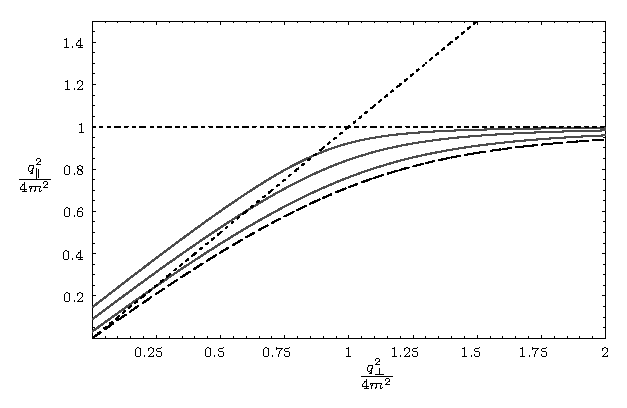
\includegraphics[width = 15cm]{fig2_1.eps}}
	\vspace*{-2mm} \caption{Законы дисперсии фотона моды 2 в сильном магнитном поле  $B/B_e = 200$  
		и нейтральной плазме ($\mu=0$) для различных значений температуры:  $T = 1$ МэВ 
		(верхняя кривая), $T = 0.5$ МэВ (средняя кривая), $T = 0.25$ МэВ (нижняя кривая). 
		Дисперсия фотона без плазмы обозначена штриховой линией.
		Диагональная штриховая линия соответствует вакуумному закону дисперсии, $q^2 = 0$. Угол
		между импульсом фотона  и направлением  магнитного поля равен 
		$\pi/2$. } 
	\label{fig:disT}
\end{figure}

Следует отметить, что полученные собственные векторы~(\ref{eq:r132}) не являются единичными, и для описания поляризационных состояний фотона удобнее использовать нормированные векторы:
%
\beq
\label{eq:epsilon}
%&&
\varepsilon_\alpha^{(1)}(q) = \frac{r^{(1)}_{\alpha}}{\sqrt{|(r^{(1)} r^{*(1)})|}} = 
\frac{(q \varphi)_\alpha}{\sqrt{q_{\mprp}^2}} \, , \quad
%\\
%\nonumber
%&&
\varepsilon_\alpha^{(2)}(q) = \frac{r^{(2)}_{\alpha}}{\sqrt{|(r^{(2)} r^{*(2)})|}} = 
\frac{(q \tilde \varphi)_\alpha}{\sqrt{q_{\mprl}^2}}.
\eeq
\noindent Здесь символы 1 и 2 соответствуют  $\|$ и $\perp$ --  поляризациям в чистом магнитном поле~\cite{Adler:1971}, $X$ - и $O$ -  модам работы~\cite{Mushtukov:2016}, и $E$ - и $O$ -  модам в замагниченной плазме~\cite{Thompson:1996}. 

Нетрудно увидеть, что полученные таким образом собственные векторы и собственные значения поляризационного 
оператора в плазме с точностью до членов порядка  $O(1/\beta^2)$ and $O(\alpha^2)$ совпадают с соответствующими величинами в  замагниченном вакууме~\footnote{Под термином <<замагниченный вакуум>>  понимается магнитное поле без плазмы.}. Такой вывод находится в согласии с результатами работы~\cite{Shabad:1988} и, для предельного случая $\omega \ll m_e$ и после необходимых преобразований: выбора продольной составляющей $\varepsilon^{(2)}_\alpha$ и перехода в систему координат, в которой вектор импульса фотона направлен вдоль оси $z$, работы~\cite{Potekhin:2004}.

Закон дисперсии фотона моды 1 в приближении $O(1/\beta^2)$ практически не отличается от вакуумного, $q^2 \simeq 0$. Действительно, из закона дисперсии для этой моды:
%
\beq
q^2 - {\cal P}^{(1)} = 0 \, 
\label{disper1}
\eeq
\noindent и формулы~(\ref{eq:kappa10}) следует, что
%
\beq
q_{\mprl}^2 = \left (1- \frac{\alpha}{3\pi} \frac{1}{1-\frac{\alpha}{3\pi} \cal V} \right) \, q_{\mprp}^2  
\simeq q_{\mprp}^2 \left (1- \frac{\alpha}{3\pi} \right)\, , 
\label{disper12}
\eeq
\noindent так что $q^2 \simeq 0$, оставаясь при этом отрицательным. Кроме того, из формулы~(\ref{eq:kappa10}) следует, что в кинематической области $q^2_{\mprl} \ll (m_e+\sqrt{m_e^2+2 \beta})^2$ собственное значение поляризационного оператора моды 1 не имеет мнимой части~\footnote{Строго говоря, мнимая часть является сильно подавленной по сравнению с реальной частью, так что такой фотон будет квазистабильным [\textcolor{red}{ссылка}].}

\begin{figure}[t]
	\centerline{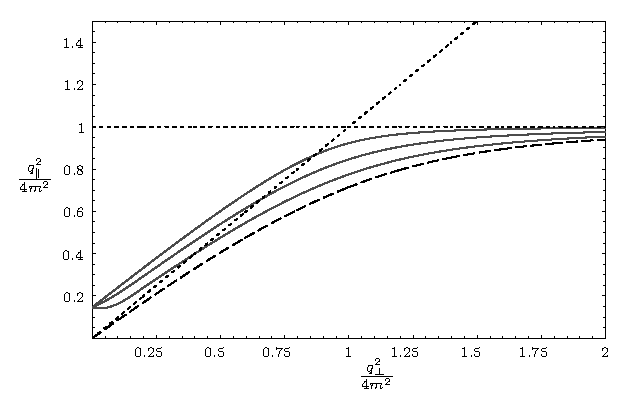
\includegraphics[width=15cm]{fig2_2.eps}} \vspace*{-2mm}
	\caption{Законы дисперсии фотона моды 2 в сильном магнитном поле  $B/B_e = 200$  
		и нейтральной плазме $(T = 1 \mbox{МэВ})$ для различных значений
		угла  между импульсом фотона  и направлением  магнитного поля
		$\theta = \pi/2$ (верхняя кривая), $\theta = \pi/6$  (средняя кривая), $\theta = \pi/12$
		(нижняя кривая).
		Дисперсия фотона без плазмы обозначена штриховой линией.
		Диагональная штриховая линия соответствует вакуумному закону дисперсии, $q^2 = 0$ \textcolor{red}{Заменить на $\mu \neq 0$}.
	}
	\label{fig:disTheta}
\end{figure}

С другой стороны, дисперсионные свойства фотона моды 2  претерпевают существенные изменения даже по сравнению с замагниченным вакуумом и, следовательно, будут оказывать дополнительное влияние на кинематику процессов с участием фотонов этой моды. На рис.~\ref{fig:disT} и~\ref{fig:disTheta} представлены законы дисперсии фотона моды 2 в замагниченной зарядово-симметричной ($\mu=0$) плазме, для различных значений температур, углов и импульса фотона, полученные как решения уравнения
%
\beq
q^2 - {\cal P}^{(2)} = 0 \, .
\label{disper}
\eeq
\noindent Как нетрудно видеть, в противоположность чистому 
магнитному полю, в плазме существует область с  $q^2 > 0$ ниже  первого  
циклотронного резонанса, определяемого условием $q^2_{\mprl} = 4 m_e^2$. 

Этот факт связан  с появлением плазменной частоты в представлении реальных электронов и позитронов среды, 
которая может быть определена из уравнения
%
\begin{equation}
\omega_{pl}^2 - {\cal P}^{(2)} (\omega_{pl}, {\mathbf k} \to 0 ) = 0.
\label{eq:omegapl}
\end{equation}
%
Для случая сильно замагниченной зарядово-симметричной нерелятивистской плазмы можно получить приближенное решение этого уравнения. В результате мы получим классическое выражение $\omega_{pl}^2 \simeq 2(4\pi \alpha n_{e})/m_e$ (множитель 2 возникает из-за равенства концентраций электронов и позитронов), где
%
\begin{eqnarray}
n_{e} \simeq \beta \sqrt{\frac{m_e T}{(2\pi)^3}}\,e^{-m_e/T}.
\label{eq:ne}
\end{eqnarray}
\noindent Таким образом, $\omega_{pl}$ для зарядово-симметричной плазмы экспоненциально подавлено. С другой стороны, для зарядово-несимметричной плазмы подавление отсутствует и $\omega_{pl}^2 \simeq (2\alpha \beta/\pi)v_F$.

Тем не менее, даже для зарядово-симметричной плазмы при температуре $T=50$ кэВ и индукции магнитного поля $B=200 B_e$ мы получаем такую оценку для плазменной частоты: $\omega_{pl} \simeq 3$ кэВ, что уже может повлиять на кинематику различных процессов с участием фотона. Например, наличие плазменной частоты приводит к возникновению порога для каналов рассеяния фотона моды 2 на электронах и позитронах плазмы, $\gamma_2 e \to \gamma_1 e$, $\gamma_2 e \to \gamma_2 e$, который отсутствует в чистом магнитном поле. А для одной из основных реакций, в которых рождаются поляризованные фотоны, -- процесса расщепления фотона на два фотона, $\gamma \to \gamma \gamma$, оно приводит к возникновению новых правил отбора по поляризациям: в области ниже порога рождения $e^+e^-$-пар, $q^2_{\mprl} = 4 m_e^2$, и в области, где $q^2 > 0$, каналы, в которых рождаются фотоны моды 2, $\gamma_2 \to \gamma_2 \gamma_2$,
$\gamma_1 \to \gamma_2 \gamma_2$ и $\gamma_1 \to \gamma_1 \gamma_2$, кинематически закрыты и становится открытым новый канал $\gamma_2 \to \gamma_1 \gamma_1$, запрещенный в магнитном поле в отсутствие плазмы.

Пропагатор фотона определяется решением следующего волнового уравнения:
\begin{eqnarray}\label{eq:WaveEq}
	\nonumber
	&& 
	(g_{\alpha \rho} \, \partial_{\mu}^2  -
	\partial_{\alpha}\partial_{\rho}) \, G^{\rho}_{\phantom{x}\beta}(x) + 
	\int d^4 x'\, {\cal P}^{(\lambda)}_{\alpha\rho} (x - x') \, 
	G^{\rho}_{\phantom{x}\beta}(x)
	\nonumber= g_{\alpha\beta}\delta^4(x),
	\label{eq:2}
\end{eqnarray}
%                                                                                         \frac{(\varphi q)_\mu}{\sqrt{q^2_\perp}}
где $\delta^4(x)=\delta(t)\delta(x)\delta(y)\delta(z)$. 

В координатном пространстве пропагатор фотона можно представить следующим 
образом:
\begin{equation}\label{eq:InvGcFourier}
	G_{\mu\nu}(x)=\int \frac{\dd^4q}{(2\pi)^4}G_{\mu\nu}(q) e^{-\ii qx}\, ,
\end{equation}
где
\begin{equation}\label{eq:GcFourier}
	G_{\mu\nu}(q)=\sum_{\lambda=1}^{3}\frac{b_\mu^{(\lambda)}b^{(\lambda)}_\nu}{(b^{(\lambda)})^2}\cdot
	 \frac{1}{q^2-{\cal P}^{(\lambda)}(q)}
\end{equation}
-- фурье-образ пропагатора.




%%%

\subsection{Резонанс на виртуальном фотоне.}
\input{Chapter4}
%%%

\subsection{Резонанс на виртуальном электроне (фермионе).}
Как было подчеркнуто в первой главе, в присутствии сильно замагниченной среды 
возможны изменения дисперсионных и поляризационных свойств фотонов. Этот факт 
может приводить к существенным изменениям кинематики процессов, в результате 
которых, например, становятся возможными такие одновершинные реакции, как однофотонное 
рождение электрон-позитронной пары $\gamma\to e^+e^-$ или поглощение фотона 
$e^{\pm}\gamma\to e^{\pm}$, которые кинематически запрещены или подавлены в 
вакууме. В выражениях для этих процессов присутствуют сингулярности, которые связаны со свойствами фазового объема (см., например,~\cite{Klepikov:1954,Sturrock:1971,Tademaru:1973,Daugherty:1983,Shabad:1988}), то возникает принципиально важная задача физически корректного определения коэффициента поглощения вблизи их окрестностей. При расчетах физических величин все резонансные бесконечные пики усреднялись~\cite{Baier:2007}, что позволило получить конечные результаты, однако такой подход является искусственным. Поэтому для устранения требуется переформулировать модель в других терминах.

Для этого в работе~\cite{Shabad:1988} предлагалось рассматривать фотон как затухающую электромагнитную волну, то есть исследовать временную зависимость волновой функции фотона. Изначально классическая задача о диссипации  в бестолкновительной плазме рассматривалось в работе~\cite{Landau:1946}, что в последствии получило название затухание Ландау. Если в классической задаче затухание связано либо с передачей энергии электромагнитного поля частицам, движущимся в фазе с волной, либо с ларморовым вращением частиц, то в квантовой электродинамике затухание квантованной электромагнитной волны определяется квантовыми процессами поглощения и рождения фотонов. Особенностью рассмотренных выше классических и квантовых процессов является их обратимость.

Для определения коэффициента затухания фотона в работе~\cite{Shabad:1988} предлагалось решать уравнение дисперсии на втором римановом листе. Однако как было отмечено в работе~\cite{MikhChist:2001}, такой метод имеет ряд недостатков. Во-первых, решения с комплексными энергиями фотона находятся на нефизических римановых листах, количество которых вообще говоря бесконечно. Это приводит к возникновению бесконечного числа решений уравнения дисперсии как с положительными, так и с отрицательными значениями мнимой части энергии. Во-вторых, в данном методе в околопороговой области предполагался экспоненциальный характер затухания электромагнитной волны, что, вообще говоря, согласно выводам авторов~\cite{MikhChist:2001}, не так. Поэтому в работе~\cite{MikhChist:2001} для исследования временного затухания электромагнитной волны во внешнем магнитном поле был рассмотрен метод, который заключается в нахождении запаздывающего решения уравнения электромагнитного поля в присутствии внешнего источника с учетом поляризации вакуума во внешнем магнитном поле. С другой стороны, в работе~\cite{MikhChist:2001} неэкспоненциальное затухание фотона рассматривалось в приближении сильного магнитного поля, когда все электроны и позитроны занимают основной уровень Ландау, однако в случае замагниченной плазмы таких исследований не проводилось, поскольку для астрофизических приложений наличие замагниченной среды является наиболее характерным фактором.


%So the probability diverges when
%the electron and the positron are created on the Landau
%levels with electron and positron momentum p3  0, see
%e.g. [6,10]. The origin of the singularity is due to the
%properties of the space volume in the lowest order of
%perturbation theory (infinitesimally narrow level). The reason why this singularity is not a pole but a branch point is
%that motion along a field is not quantized.

В данном разделе рассматривается затухание фотона в сильно замагниченной плазме $\beta \gg T^2$
и нулевом химическом потенциале $\mu = 0$ посредством изменения его состояния за счет процессов $\gamma e^\pm\to e^\pm$, $\gamma \to e^+e^-$. Будет использоваться метод, применяемый в теории поля при конечных температурах и в физике плазмы~\cite{Boyan}, развитый на случай сильного магнитного поля в~\cite{MikhChist:2001} и адаптированный к ситуации сильно замагниченной плазмы.

\subsection{Распространение фотона в замагниченной плазме}

Для описания эволюции электромагнитной волны ${\cal A}_{\alpha}(x)$, где $x_\mu = (t, {\bf x})$, 
во времени воспользуемся методикой, которая была использована еще в классической задаче~\cite{Landau:1946} и развита  в работе~\cite{MikhChist:2001} для квантовой электродинамики с учетом только магнитного поля без плазмы. Данная методика заключается в определении реакции системы 
(${\cal A}_{\alpha}(x)$ и замагниченной плазмы) на внешний источник~\cite{Kirzhnits:1987}, создающий начальное состояние, который адиабатически включается 
при $t = - \infty$ и в момент времени $t = 0$ выключается. При $t > 0$
электромагнитная волна в плазме будет эволюционировать самостоятельно. Для простоты будем рассматривать эволюцию монохроматической волны, поэтому 
функцию источника, удовлетворяющую вышесказанным условиям, удобно выбрать следующим образом:
%
\beq
{\cal J}_{\alpha}(x) = j_{\alpha}\,e^{i \,{\bf k} {\bf x}}\,
e^{ \varepsilon t}\, \theta(- t), \,\,\, \varepsilon \to 0^+,
\label{eq:1}
\eeq
где $j_{\alpha} = (0, {\bf j}),\,\,{\bf j} \cdot {\bf k} = 0$ – закон сохранения тока. Вообще говоря, в замагниченной плазме из-за наличия анизотропии решение задачи о распространении фотона под произвольным углом к магнитному полю представляет значительные трудности. Поэтому в качестве упрощения рассмотрим частный случай, когда фотоны распространяются поперек магнитного поля так, что $k_z=0$. Зависимость ${\cal A}_{\alpha}(x)$ от времени  определяется уравнением
%
\begin{eqnarray}\label{eq:WaveEq}
%\nonumber
%&& 
(g_{\alpha \beta} \, \partial_{\mu}^2  -
\partial_{\alpha}\partial_{\beta}) \, {\cal A}_{\beta}(x) + 
%\nonumber \\
%&&+ 
\int d^4 x'\, {\cal P}_{\alpha \beta} (x - x') \, {\cal A}_{\beta}(x')
= {\cal J}_{\alpha}(x),
\label{eq:2}
\end{eqnarray}
%                                                                                         \frac{(\varphi q)_\mu}{\sqrt{q^2_\perp}}
где ${\cal P}_{\alpha \beta} (x - x')$ -- поляризационный оператор фотона в магнитном поле и плазме. $q^{\mu} = (q_0,\, {\bf k})$ -- 4-вектор импульса фотона.

% Следует отметить, что в общем случае поляризационный оператор зависит от каждой координаты $x$ и $x'$ в отдельности. Однако, если рассматриваются процессы на достаточно малых расстояниях и временах, то среду в таком случае можно считать однородной. Тогда поляризационный оператор будет зависеть от разности $x-x'$.


Запаздывающее решение уравнения~(\ref{eq:WaveEq}) можно представить в следующем виде:

\begin{equation}\label{eq:RetSol}
	{\cal A}_\alpha(x)=\int \dd^4 x' G^R_{\alpha \beta}(x-x'){\cal J}_\beta(x')\, ,
\end{equation}
где $G^R_{\alpha \beta}(x-x')$ -- запаздывающая функция Грина (см., например~\cite{Landau:2001}).

Следуя работе~\cite{MikhChist:2001}, аналогично процессу затухания в магнитном поле воспользуемся следующим соотношением между запаздывающей $G^R_{\alpha\beta}(x-x')$ и причинной $G^C_{\alpha\beta}(x-x')$ функциями Грина:

\begin{equation}\label{eq:RetCasualGreen}
G^R_{\alpha\beta}(x-x')= 2 \mathrm{Re} \left[G^C_{\alpha\beta}(x-x')\right]\theta(t-t')\, .
\end{equation}

Аналогично магнитному полю разложим функцию Грина по собственным векторам $r_\alpha^{(\lambda)}$ поляризационного оператора в замагниченной плазме:
\begin{equation}\label{eq:InvGcFourier}
	G^C_{\alpha\beta}(x)=\int \frac{\dd^4q}{(2\pi)^4}G^C_{\alpha \beta}(q) e^{-\ii qx}\, ,
\end{equation}
\begin{equation}\label{eq:GcFourier}
	G^C_{\alpha\beta}(q)=\sum_{\lambda=1}^{3}\frac{r_\alpha^{(\lambda)}r^{(\lambda)}_\beta}{(r^{(\lambda)})^2}\cdot \frac{1}{q^2-{\cal P}^{(\lambda)}(q)}\, ,
\end{equation}
где ${\cal P}^{(\lambda)}(q)$ -- собственные значения поляризационного оператора в замагниченной плазме.


Как было отмечено в разделе~\ref{Ch:Photon}, в случае сильно замагниченной плазмы~$\beta\gg T^2$ и $\mu=0$ собственные вектора поляризационного оператора фотона приближенно будут такими же, как и в чистом магнитном поле:

\begin{equation}\label{eq:ASolve}
	{\cal A}_\alpha(x) = 2 e^{i \mathbf{kx}} \mathrm{Re} \sum_{\lambda=1}^3 \int\frac{\dd q_0}{2\pi i}\frac{\varepsilon_\alpha^{(\lambda)}(\varepsilon^{(\lambda)} j)}{(\varepsilon^{(\lambda)})^2}\frac{e^{-i q_0 t}}{(q_0-i\varepsilon)(q_0^2-\mathbf{k}^2-{\cal P}^{(\lambda)}(q))}\, .
\end{equation}


В силу линейного характера уравнения~(\ref{eq:WaveEq}), решение~(\ref{eq:ASolve}) для двух возможных поляризаций можно представить в виде:
\begin{equation}\label{eq:ASoveDivide}
	{\cal A}_\alpha(x)={\cal A}^{(1)}_\alpha(x)+{\cal A}^{(2)}_\alpha(x)\, ,
\end{equation}
где 
%
\begin{eqnarray}                        		
{\cal A}^{(\lambda)}_{\alpha} (x) = V^{(\lambda)}_\alpha (0, {\bf x}) \, \text{Re} F^{(\lambda)} (t) \, ,
\label{eq:V}
\end{eqnarray}
\begin{eqnarray}
V^{(\lambda)}_\alpha (0, {\bf x}) = 2\, e^{ i\, {\bf k x}} \, 
\varepsilon^{(\lambda)}_\alpha \, (\varepsilon^{(\lambda)} j)\, .
\label{eq:partialV}
\end{eqnarray}
%
%\beq
%V^{(2)}_\alpha (0, {\bf x}) = 2\, e^{ i\, {\bf k x}} \, \varepsilon^{(2)}_\alpha \, \frac{(q \tilde \varphi j)}{\sqrt{q^2_{\mprl}}} \, .
%\label{eq:partialV2}
%\eeq
%Для дальнейшего анализа, контур интегрирования удобно
%преобразовать в контур, изображенный на рис.11. 

Как следует из~(\ref{eq:ASoveDivide}) и~(\ref{eq:ASolve}) характер распространения фотона в сильно замагниченной плазме будет полностью определяться функцией $F^{(\lambda)} (t)$, которая имеет мледующий вид Фурье-интеграла:

\begin{equation}\label{eq:FullIntegrate}
	F^{(\lambda)}(t)=\int_C\frac{dq_0}{2\pi \ii}\frac{e^{-\ii q_0 t}}{(q_0-\ii \varepsilon)(q_0^2-\vec{k}^2-{\cal P}^{(\lambda)}(q))}.
\end{equation}

	\begin{figure}[t]\centering
		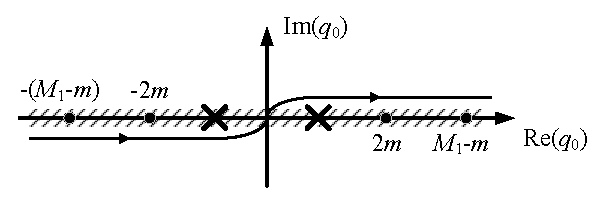
\includegraphics[scale=1.5]{PathIntegrateMode2.eps}
		\caption{Контур интегрирования по $q_0$ в~(\ref{eq:FullIntegrate}) для моды 2. Штрихами показана область нестабильности фотона. Крестиком обозначен полюс, соответствующий $q_0=\omega$ -- вещественному собственному значению поляризационного оператора.}\label{fig:FullPathIntegr}.
	\end{figure}

Контур интегрирования $C$ определяется согласно аналитическим свойствам подынтегрального выражения. В частности, в точке $q_0=\omega$ подынтегральное выражение~(\ref{eq:FullIntegrate}) имеет полюс, который соответствует уравнению дисперсии:

\begin{equation}
	\omega^2 - \vec{k}^2 - {\cal P^{(\lambda)}}(q)=0.
\end{equation}

\begin{center}
	\begin{figure}[t!]\centering
		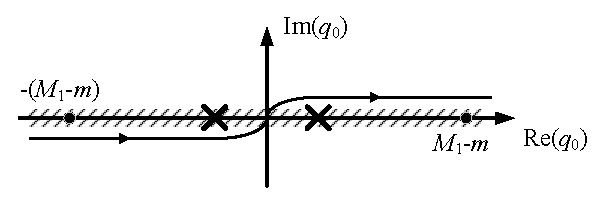
\includegraphics[scale=1.5]{PathIntegrateMode1.eps}
		\caption{Контур интегрирования по $q_0$ в~(\ref{eq:FullIntegrate}) для моды 1. Штрихами показана область нестабильности фотона. Крестиком обозначен полюс, соответствующий $q_0=\omega$ -- вещественному собственному значению поляризационного оператора, точками обозначены полюса.} \label{fig:FullPathIntegrMode1}
	\end{figure}
\end{center}

С другой стороны, как было показано в работе~\cite{MikhChist:2001}, собственные значения поляризационного оператора как в магнитном поле, так и в замагниченной плазме помимо полюсов $q_{\mprl}^2=(M_n\pm M_\ell)^2$, отмеченных в разделе~\ref{Ch:Compton}, также имеют разрезы, которые связаны с распадом фотона на $e^+e^-$-пару и переходом электрона на другие уровни Ландау, т. е. соответствуют областям нестабильности фотона, поэтому с учетом этих особенностей  контур интегрирования может быть определен, как показано на~рис.~\ref{fig:FullPathIntegrMode1}~и~\ref{fig:FullPathIntegr}.

Следует отметить, что в сильно замагниченной плазме в кинематической области $q_0<2m$ мнимая часть поляризационного оператора для обеих мод пренебрежимо мала по сравнению с реальной частью (влияние резонансов отсутствует), поэтому для удобства контур интегрирования как для фотона моды~1, так и для фотона моды 2 можно преобразовать согласно рис.~\ref{fig:PathIntegr}. Таким образом, интеграл~(\ref{eq:FullIntegrate}) можно представить в виде двух слагаемых
\begin{eqnarray}
F^{(\lambda)}(t) = F^{(\lambda)}_{pole}(t) + F^{(\lambda)}_{cut}(t),
\label{eq:19}
\end{eqnarray}
%
первое из которых определяется вычетом в точке $q_0 = \omega$, являющейся
решением уравнения дисперсии $q^2 - {\cal P}^{(\lambda)}(q) = 0$ в кинематической области, где собственное 
значение поляризационного оператора фотона ${\cal P}^{(\lambda)}(q)$ -- вещественно. 

%Оно соответствует незатухающему
%решению в области $\omega < 2 m$~\cite{Shab}.
Второе слагаемое определяет зависимость потенциалов ${\cal A}^{(\lambda)}_\alpha(x)$ от времени
в области $q_0>2m$ и имеет вид
фурье-интеграла:
%
\begin{eqnarray}
F^{(\lambda)}_{cut}(t) &=& \int \limits_{- \infty}^{\infty} \frac{dq_0}{2 \pi}\,
F^{(\lambda)}_{cut}(q_0)e^{- i q_0 t},
\label{eq:20} 
\\
F^{(\lambda)}_{cut}(q_0) &\simeq& 
\frac{2 \,\theta (q_0  -  2 m)\,I^{(\lambda)}}
{q_0\,([ q_0^2 - {\bf k}^2 - R^{(\lambda)}]^2 + [I^{(\lambda)}]^2)},
\label{eq:21}
\end{eqnarray}
%
где $R \equiv \text{Re} {\cal P}^{(\lambda)}(q_0)$  – реальная, $I \equiv  - \text{Im} {\cal P}^{(\lambda)}(q_0 + i \varepsilon)$ – мнимая 
части поляризационного оператора фотона в замагниченной плазме.

Мнимая часть поляризационного оператора может быть получена из коэффициента  
поглощения фотона и представлена в следующем виде:
\begin{eqnarray}
W^{(\lambda)}_{abs} = W_{\gamma^{(\lambda)} \to e^+ e^-} + W_{\gamma^{(\lambda)} e^{\pm} \to e^{\pm}} \, .
\label{eq:Wabs}
\end{eqnarray}
где $W_{\gamma^{(\lambda)} \to e^+ e^-}$ -- коэффициент поглощения фотона в процессе однофотонного рождения электрон-позитронной пары, $W_{\gamma^{(\lambda)} e^{\pm} \to e^{\pm}}$ -- коэффициент поглощения фотона в процессе поглощения фотона электроном.

\begin{figure}[t]\centering
	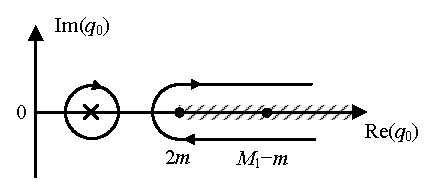
\includegraphics[scale=1.5]{PathIntegrate2Gl.eps}
	\caption{Контур интегрирования по $q_0$ в~(\ref{eq:20}) для мод $\lambda = 1,2$. Штриховой линией показана область, где мнимая часть поляризационного оператора двух возможных мод $\lambda = 1,2$ существенна. Остальные обозначения аналогичны~рис.~\ref{fig:FullPathIntegr}.}\label{fig:PathIntegr}
\end{figure}

С учетом процессов излучения фотонов, (\ref{eq:Wabs}) может быть представлена в следующей форме (см., например,~\cite{Shabad:1988, Rumyantsev:2017,Weldon:1983}): 
\begin{eqnarray}\label{eq:Ilambda}
I^{(\lambda)}=\text{Im} {\cal P}^{(\lambda)} =  -2 q_0 [1-\exp (-q_0/T)] W^{(\lambda)}_{abs} \, . 
\label{eq:ImP}
\end{eqnarray}

Реальная часть 
поляризационного оператора может быть восстановлена по его мнимой части с помощью дисперсионного соотношения с одним 
вычитанием:
%
\beq 
R^{(\lambda)}=\textrm{Re}{\cal P}^{(\lambda)} (t) = \int \limits_0^\infty \frac{\textrm{Im}({\cal P}^{(\lambda)} (t'))\,dt'}{t'-t-i o} - \textrm{Re}{\cal P}^{(\lambda)} (0)\,, \qquad  t = q^2_0 \, .
\label{eq:Disp}
\eeq

Следует отметить, что в поставленной задаче рассматриваются процессы только до второго циклотронного резонанса $q_0=M_1-m$, поэтому те же процессы с другими уровнями Ландау вклада не дают.
Выражения (\ref{eq:20})-(\ref{eq:Wabs}) с учетом (\ref{eq:Disp}) решают задачу 
о нахождении временной зависимости волновой функции фотона  в присутствии сильно 
замагниченной плазмы. 

В работе~\cite{Shabad:1988}
предполагался экспоненциальный характер затухания с декрементом затухания, равным мнимой части энергии фотона, полученным из решения уравнения дисперсии на втором римановом листе. Анализ  аналитических свойств фурье-образа $F^{(\lambda)}_{cut}(q_0)$ показывает, что характер временного затухания волновой функции в общем случае является неэкспоненциальным. Тем не менее на протяжении некоторого характерного отрезка времени $(\sim [W^{(\lambda)}_{abs}]^{-1})$
зависимость волновой функции от времени можно приближенно описать как 
экспоненциально затухающие гармонические колебания:
%
\begin{equation}\label{eq:ApproxA}
{\cal A}^{(\lambda)}_\mu(t) \sim e^{- \gamma^{(\lambda)}_\text{eff} \, t/2} \cos 
(\omega^{(\lambda)} t + \phi_0).
\end{equation}
%
Здесь $\omega^{(\lambda)}$ и $\gamma^{(\lambda)}_\text{eff}$ -- эффективная 
частота и коэффициент  
поглощения фотона моды $\lambda$ соответственно, которые должны быть найдены с использованием 
(\ref{eq:20})--(\ref{eq:Wabs}) для каждого значения импульса ${\bf k}$, что определяет эффективный 
закон дисперсии фотона в области его нестабильности.


\subsection{Численный анализ}


\begin{figure}[t]\centering
	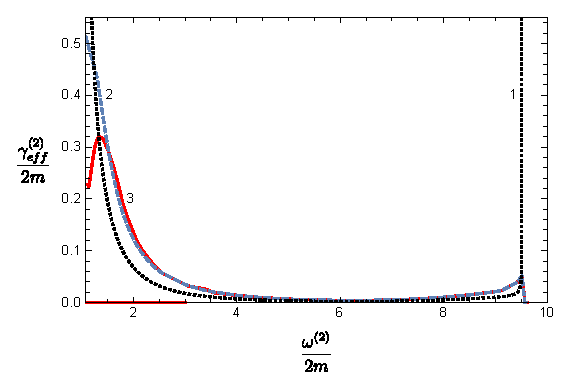
\includegraphics[scale=0.8]{mode2.eps}
	\caption{\label{fig:fig2}Зависимость ширины распада фотона моды 2 от частоты в припороговых областях при $B=200 B_e$, $T=1$ МэВ и $ \mu=0 $. Линия $ {\it 1} $ - коэффициент поглощения фотона $ W ^ {(1)}_{abs} $,
		% в процессах $ \ gamma \ to e ^ + e ^ - $ и $ \ gamma e ^ { \ pm} \ to e ^ {\ pm} $,
		вычисленный в древесном приближении и содержащий корневые особенности; линия $ {\it 2} $ -- ширина распада, полученная из комплексного решения дисперсионного уравнения на втором римановом листе~\cite{Shabad:1988}; линия $ {\it 3} $ соответствует ширине затухания $ \gamma^{(1)}$, вычисленной на основе приближения~(\ref{eq:ApproxA}).}\label{fig:DampMode2}
\end{figure}

Для астрофизических приложений полезно вычислить величину $\gamma_\text{eff}$, которая определяет интенсивность поглощения 
$\gamma$-квантов в замагниченной плазме за счет  процессов $\gamma \to e^+ e^-$  и $\gamma e^{\pm} \to e^{\pm}$.
Обычно в астрофизике  используют выражение для коэффициента поглощения,
полученное на основе  вероятности распада  $ \gamma \to e^+ e^-$. Однако в околопороговой области эти выражения
содержат корневые сингулярности (см. например~\cite{HBG:1997}), которые были отмечены во введении к данной главе. 

Наш анализ показывает, (см. рис.~\ref{fig:DampMode1} и~\ref{fig:DampMode2}),
что вычисление коэффициента  поглощения с учетом неэкспоненциального характера 
затухания приводит к конечному выражению для коэффициента  поглощения фотона в окрестности резонансов 
$q_0 = (\sqrt{m^2+2 \beta} - m )$ как для фотона моды 2, так и для фотона моды 1. Исходя из рис. \ref{fig:DampMode1} можно сделать вывод, что фотон моды 1 является квазистабильным в областях $q_0<7$ МэВ и $q_0>(\sqrt{m^2+2 \beta} - m)\simeq 9.5$~МэВ. С другой стороны, фотон неустойчив в области, близкой в окрестности резонансов $q_0 = (\sqrt{m^2+2 \beta} - m )$. Фотон моды 2 можно считать квазиустойчивым в области $q_0<4m$ и $q_0>(\sqrt{m^2+2 \beta} - m)$. Коэффициент затухания фотона, полученный из результатов работы~\cite{Shabad:1988}, является завышенным в околопороговой области по сравнению с результатами, полученными с помощью аппроксимации~(\ref{eq:ApproxA}). Однако существует область энергий фотона ($2.5\lesssim q_0\lesssim 8.5$ МэВ для фотона моды 2 и $q_0\lesssim8.7$ МэВ для фотона моды 1), где коэффициенты поглощения, полученные из результатов работы~\cite{Shabad:1988} и с помощью аппроксимации~(\ref{eq:ApproxA}) совпадают.


\begin{figure}[t]\centering
	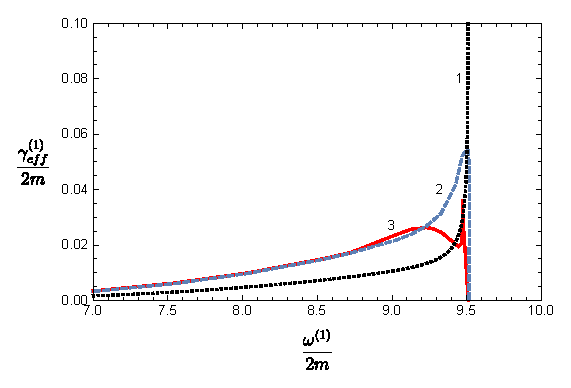
\includegraphics[scale=0.8]{mode1.eps}
	\caption{\label{fig:fig1}Зависимость ширины распада фотона моды 1 от частоты в припороговых областях при $B=200 B_e$, $T=1$ МэВ и $ \mu=0 $. Линия $ {\it 1} $ - коэффициент поглощения фотона $ W ^ {(1)}_{abs} $,
		% в процессах $ \ gamma \ to e ^ + e ^ - $ и $ \ gamma e ^ { \ pm} \ to e ^ {\ pm} $,
		вычисленный в древесном приближении и содержащий корневые особенности; линия $ {\it 2} $ - ширина распада, полученная из комплексного решения дисперсионного уравнения на втором римановом листе~\cite{Shabad:1988}; линия $ {\it 3} $ соответствует ширине затухания $ \gamma^{(1)}$, вычисленной на основе приближения~(\ref{eq:ApproxA}).}\label{fig:DampMode1}
\end{figure}

\begin{figure}[t!]\centering
	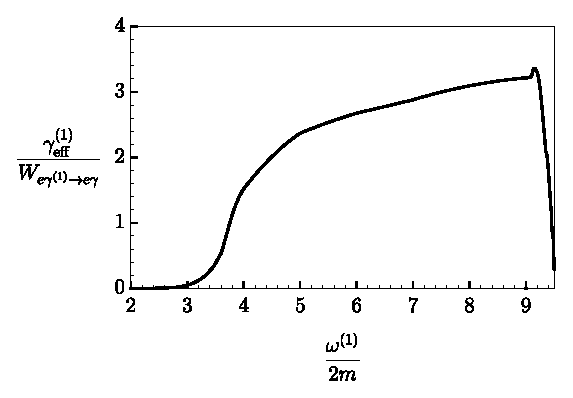
\includegraphics[scale=1.3]{CompareDampAndCompton.eps}
	\caption{\label{fig:ComptonandDamp} Отношение коэффициента затухания фотона $\gamma_{eff}^{(1)}$ к коэффициенту поглощения фотона в процессе $e\gamma^{(1)}\to e\gamma$ при $B=200B_e$ и $T=1$ МэВ}
\end{figure}
\clearpage
\begin{figure}[t!]\centering
	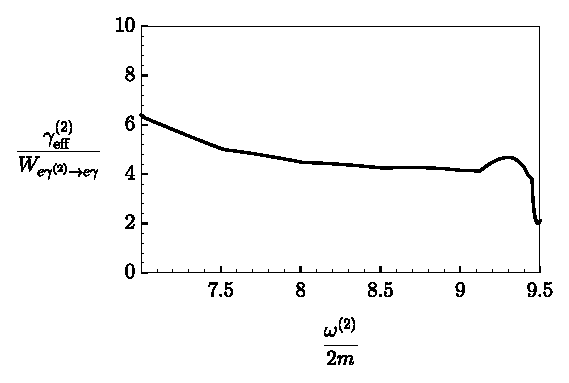
\includegraphics[scale=1.3]{CompareDampAndCompton2.eps}
	\caption{\label{fig:ComptonandDamp2} Отношение коэффициента затухания фотона $\gamma_\text{eff}^{(2)}$ к коэффициенту поглощения фотона в процессе $e\gamma^{(2)}\to e\gamma$ при $B=200B_e$ и $T=1$ МэВ}
\end{figure}


На основе полученных результатов представляет интерес рассмотреть задачу о возможности формировании комптоновского процесса при условии затухания фотона. Для этого удобно вычислить отношение коэффициента затухания фотона к коэффициенту поглощения фотона $e\gamma^{(1)}\to e\gamma$  (см. рис. \ref{fig:ComptonandDamp}), полученном в главе 2 и который определяет время его формирования. Как видно из рисунка~\ref{fig:ComptonandDamp}, комптоновский процесс, несмотря на малый фактор $\alpha$, успевает формироваться при энергиях фотона $\omega\lesssim3$ МэВ. Для фотона моды 2 комптоновский процесс формируется только в области энергий фотона $\omega\lesssim1$ МэВ. В области энергий $\omega>3$ МэВ для моды 1 и $\omega>1$ МэВ фотоны будут эффективно затухать, и комптоновский процесс, по-видимому, не успевает сформироваться. Для моды 2 (см. рис.~\ref{fig:ComptonandDamp2}) даже с учетом области квазистабильности (вдали от порогов), комптоновский процесс будет формироваться только при энергиях фотона~$\omega<1$~МэВ.

Таким образом, коэффициенты поглощения фотона в комптоновском процессе для двух возможных каналов рассеяния $e\gamma^{(1)}  \to e\gamma^{(1)}$ и $e\gamma^{(1)}  \to e\gamma^{(2)}$, несмотря на резонансный характер, целесообразно рассматривать лишь вдали от циклотронных резонансах, поэтому для анализа комптоновского процесса при высоких температурах $T\simeq 1$ МэВ и магнитных полях $B=200 B_e$ достаточно использовать разложение по обратным степеням напряженности магнитного поля~\cite{Chistyakov:2009}. Каналы же рассеяния $e\gamma^{(2)}  \to e\gamma^{(1)}$  и $e\gamma^{(2)}  \to e\gamma^{(2)}$ в области резонанса рассматривать нецелесообразно, так как комптоновский процесс не успевает сформироваться для энергий фотона $\omega\gtrsim 2m$.

\subsection{Выводы}
Исследован процесс распространения квантованной электромагнитной волны в сильно замагниченной, зарядово-симметричной плазме. С учетом изменения дисперсионных свойств фотона в магнитном поле и плазме было установлено, что, аналогично случаю чистого магнитного поля процесс затухания фотона
в замагниченной плазме имеет неэкспоненциальный характер. 

Для характерного отрезка времени $\sim [W^{{(\lambda)}}_{abs}]^{-1}$ была использована аппроксимация экспоненциально затухающими колебаниями. В этом случае было
показано, что коэффициент поглощения фотона в околопороговой области меньше по сравнению с известными в литературе результатами. Также, следуя данной аппроксимации, были построены дисперсионные кривые, которые и для моды 1, и для моды 2 близки к вакуумным кривым, за исключением околопороговых областей. Полученные результаты согласуются с выводами работы~\cite{Shabad:1988}.

Бёыл выполнен анализ возможности формирования комптоновского процесса в условиях нестабильности фотона за счет процесса поглощения электроном $e^\pm\gamma\to e^\pm$ и распада на электрон-позитронную пару $\gamma\to e^+e^-$. Несмотря на малый фактор $\alpha$, комптоновский процесс преобладает над процессами распада и поглощения в области низких энергий фотона ($\omega<3$ МэВ при $T=1$ МэВ и $B =200B_e$). С другой стороны, даже с учетом резонанса на виртуальном электроне, фотоны как моды 1, так и моды~2 в пределе сильного магнитного поля $B=200 B_e$ и температуре $T=1$ МэВ эффективно затухают в резонансной области.

%%%%

\subsection{Резонанс на виртуальном электроне и виртуальном фотоне.}
Как было подчеркнуто в первой главе, в присутствии сильно замагниченной среды 
возможны изменения дисперсионных и поляризационных свойств фотонов. Этот факт 
может приводить к существенным изменениям кинематики процессов, в результате 
которых, например, становятся возможными такие реакции, как однофотонное 
рождение электрон-позитронной пары $\gamma\to e^+e^-$ или поглощение фотона 
$e^{\pm}\gamma\to e^{\pm}$, которые кинематически запрещены или подавлены в 
вакууме. С другой стороны, анализ кинематики этих реакций говорит о том, что 
они будут давать определенный вклад в процессы изменения состояния фотона как 
затухающей квантованной электромагнитной волны. Поэтому представляет отдельный 
интерес рассмотреть сам процесс затухания фотона за счет реакций поглощения 
фотона электроном (позитроном)
$\gamma e^{\pm} \to e^{\pm}$ и рождения электрон-позитронных пар $\gamma \to e^+ e^-$, которые являются важными в астрофизике замагниченных нейтронных звезд~\cite{Kostenko:2018,Philippov_2020}. 

Процесс рождения электрон-позитронной пары  в магнитном поле в древесном приближении был рассмотрен в ряде работ~(см., например,~\cite{Klepikov:1954,Sturrock:1971,Tademaru:1973,Daugherty:1983,Shabad:1988}). Однако, как подчеркивается в работе~\cite{Shabad:1988}, факт наличия корневых сингулярностей в вероятности процесса $\gamma\to e^+e^-$ указывает на то, что эту величину, вообще говоря, нельзя интерпретировать как коэффициент затухания фотона вблизи их окрестности, соответствующих резонансным областям. Поэтому для решения этой задачи в работе~\cite{Shabad:1988} предлагалось определять коэффициент затухания фотона, решая уравнение дисперсии на втором римановом листе.  Как было отмечено в работе~\cite{MikhChist:2001}, такой метод имеет ряд недостатков. Во-первых, решения с комплексными энергиями фотона находятся на нефизических римановых листах, количество которых вообще говоря бесконечно. Это приводит к возникновению бесконечного числа решений уравнения дисперсии как с положительными, так и с отрицательными значениями мнимой части энергии. Во-вторых, в данном методе в околопороговой области предполагался экспоненциальный характер затухания электромагнитной волны, что, вообще говоря, согласно выводам авторов~\cite{MikhChist:2001}, не так. Поэтому в работе~\cite{MikhChist:2001} для исследования временного затухания электромагнитной волны во внешнем магнитном поле был рассмотрен метод, который заключается в нахождении запаздывающего решения уравнения электромагнитного поля в присутствии внешнего источника с учетом поляризации вакуума во внешнем магнитном поле. С другой стороны, в работе~\cite{MikhChist:2001} неэкспоненциальное затухание фотона рассматривалось в приближении сильного магнитного поля, когда все электроны и позитроны занимают основной уровень Ландау, однако в случае замагниченной плазмы таких исследований не проводилось, поскольку для астрофизических приложений наличие замагниченной среды является наиболее характерным фактором.

В данной главе рассматривается затухание фотона в сильно замагниченной плазме $\beta \gg T^2$
 и нулевом химическом потенциале $\mu = 0$ посредством изменения его состояния за счет процессов $\gamma e^\pm\to e^\pm$, $\gamma \to e^+e^-$. Будет использоваться метод, применяемый в теории поля при конечных температурах и в физике плазмы~\cite{Boyan}, развитый на случай сильного магнитного поля в~\cite{MikhChist:2001} и адаптированный к ситуации сильно замагниченной плазмы.

\section{Распространение фотона в замагниченной плазме}

Для описания эволюции электромагнитной волны ${\cal A}_{\alpha}(x)$, где $x_\mu = (t, {\bf x})$, 
во времени воспользуемся методикой, подробно изложенной в~\cite{MikhChist:2001} для случая магнитного поля. Данная методика заключается в определении реакции системы 
(${\cal A}_{\alpha}(x)$ и замагниченной плазмы) на внешний источник~\cite{Kirzhnits:1987}, создающий начальное состояние, который адиабатически включается 
при $t = - \infty$ и в момент времени $t = 0$ выключается. При $t > 0$
электромагнитная волна в плазме будет эволюционировать самостоятельно. Для простоты будем рассматривать эволюцию монохроматической волны, поэтому 
функцию источника удобно выбрать в том же виде, что и для сильного магнитного поля:
%
\beq
{\cal J}_{\alpha}(x) = j_{\alpha}\,e^{i \,{\bf k} {\bf x}}\,
e^{ \varepsilon t}\, \theta(- t), \,\,\, \varepsilon \to 0^+,
\label{eq:1}
\eeq
где $j_{\alpha} = (0, {\bf j}),\,\,{\bf j} \cdot {\bf k} = 0$ – закон сохранения тока. Вообще говоря, в замагниченной плазме из-за наличия анизотропии решение задачи о распространении фотона под произвольным углом к магнитному полю представляет значительные трудности. Поэтому в качестве упрощения рассмотрим частный случай, когда фотоны распространяются поперек магнитного поля так, что $k_z=0$. Зависимость ${\cal A}_{\alpha}(x)$ от времени  определяется уравнением
%
\begin{eqnarray}\label{eq:WaveEq}
%\nonumber
%&& 
(g_{\alpha \beta} \, \partial_{\mu}^2  -
\partial_{\alpha}\partial_{\beta}) \, {\cal A}_{\beta}(x) + 
%\nonumber \\
%&&+ 
\int d^4 x'\, {\cal P}_{\alpha \beta} (x - x') \, {\cal A}_{\beta}(x')
= {\cal J}_{\alpha}(x),
\label{eq:2}
\end{eqnarray}
%                                                                                         \frac{(\varphi q)_\mu}{\sqrt{q^2_\perp}}
где ${\cal P}_{\alpha \beta} (x - x')$ -- поляризационный оператор фотона в магнитном поле и плазме. $q^{\mu} = (q_0,\, {\bf k})$ -- 4-вектор импульса фотона.

% Следует отметить, что в общем случае поляризационный оператор зависит от каждой координаты $x$ и $x'$ в отдельности. Однако, если рассматриваются процессы на достаточно малых расстояниях и временах, то среду в таком случае можно считать однородной. Тогда поляризационный оператор будет зависеть от разности $x-x'$.

Запаздывающее решение уравнения~(\ref{eq:WaveEq}) можно представить в следующем виде:

\begin{equation}\label{eq:RetSol}
	{\cal A}_\alpha(x)=\int \dd^4 x' G^R_{\alpha \beta}(x-x'){\cal J}_\beta(x')\, ,
\end{equation}
где $G^R_{\alpha \beta}(x-x')$ -- запаздывающая функция Грина (см., например~\cite{Landau:2001}).

Следуя работе~\cite{MikhChist:2001}, аналогично процессу затухания в магнитном поле воспользуемся следующим соотношением между запаздывающей $G^R_{\alpha\beta}(x-x')$ и причинной $G^C_{\alpha\beta}(x-x')$ функциями Грина:

\begin{equation}\label{eq:RetCasualGreen}
G^R_{\alpha\beta}(x-x')= 2 \mathrm{Re} \left[G^C_{\alpha\beta}(x-x')\right]\theta(t-t')\, .
\end{equation}

\begin{center}
	\begin{figure}[t!]\centering
		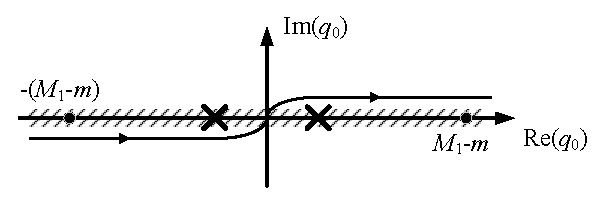
\includegraphics[scale=1.5]{PathIntegrateMode1.eps}
		\caption{Контур интегрирования по $q_0$ в~(\ref{eq:FullIntegrate}) для моды 1. Штрихами показана область нестабильности фотона. Крестиком обозначен полюс, соответствующий $q_0=\omega$ -- вещественному собственному значению поляризационного оператора, точками обозначены полюса.} \label{fig:FullPathIntegrMode1}
	\end{figure}
\end{center}

Аналогично магнитному полю разложим функцию Грина по собственным векторам $r_\alpha^{(\lambda)}$ поляризационного оператора в замагниченной плазме (см. приложение~\ref{app3}):
\begin{equation}\label{eq:InvGcFourier}
	G^C_{\alpha\beta}(x)=\int \frac{\dd^4q}{(2\pi)^4}G^C_{\alpha \beta}(q) e^{-\ii qx}\, ,
\end{equation}
\begin{equation}\label{eq:GcFourier}
	G^C_{\alpha\beta}(q)=\sum_{\lambda=1}^{3}\frac{r_\alpha^{(\lambda)}r^{(\lambda)}_\beta}{(r^{(\lambda)})^2}\cdot \frac{1}{q^2-{\cal P}^{(\lambda)}(q)}\, ,
\end{equation}
где ${\cal P}^{(\lambda)}(q)$ -- собственные значения поляризационного оператора в замагниченной плазме.

Далее, подставляя выражение~(\ref{eq:RetSol}) в (\ref{eq:WaveEq}) с учетом~(\ref{eq:RetCasualGreen})--(\ref{eq:GcFourier}), получим следующий результат:
\begin{equation}\label{eq:ASolvePlasma}
	{\cal A}_\alpha(x) = 2 e^{i \mathbf{kx}} \mathrm{Re} \sum_{\lambda=1}^3 \int\frac{\dd q_0}{2\pi i}\frac{r_\alpha^{(\lambda)}(r^{(\lambda)} j)}{(r^{(\lambda)})^2}\frac{e^{-i q_0 t}}{(q_0-i\varepsilon)(q_0^2-\mathbf{k}^2-{\cal P}^{(\lambda)}(q))}\, .
\end{equation}

Как было отмечено в главе 1 и показано в приложении~\ref{app3}, в случае сильно замагниченной плазмы $\beta\gg T^2$ и $\mu=0$ собственные вектора поляризационного оператора фотона приближенно будут такими же, как и в чистом магнитном поле, поэтому перепишем~(\ref{eq:ASolve}) в виде:

\begin{equation}\label{eq:ASolve}
	{\cal A}_\alpha(x) = 2 e^{i \mathbf{kx}} \mathrm{Re} \sum_{\lambda=1}^3 \int\frac{\dd q_0}{2\pi i}\frac{\varepsilon_\alpha^{(\lambda)}(\varepsilon^{(\lambda)} j)}{(\varepsilon^{(\lambda)})^2}\frac{e^{-i q_0 t}}{(q_0-i\varepsilon)(q_0^2-\mathbf{k}^2-{\cal P}^{(\lambda)}(q))}\, .
\end{equation}

В силу линейного характера уравнения~(\ref{eq:WaveEq}), решение~(\ref{eq:ASolve}) для двух возможных поляризаций можно представить в виде:
\begin{equation}\label{eq:ASoveDivide}
	{\cal A}_\alpha(x)={\cal A}^{(1)}_\alpha(x)+{\cal A}^{(2)}_\alpha(x)\, ,
\end{equation}
где 
%
\begin{eqnarray}                        		
{\cal A}^{(\lambda)}_{\alpha} (x) = V^{(\lambda)}_\alpha (0, {\bf x}) \, \text{Re} F^{(\lambda)} (t) \, ,
\label{eq:V}
\end{eqnarray}
\begin{eqnarray}
V^{(\lambda)}_\alpha (0, {\bf x}) = 2\, e^{ i\, {\bf k x}} \, 
\varepsilon^{(\lambda)}_\alpha \, (\varepsilon^{(\lambda)} j)\, .
\label{eq:partialV}
\end{eqnarray}
%
%\beq
%V^{(2)}_\alpha (0, {\bf x}) = 2\, e^{ i\, {\bf k x}} \, \varepsilon^{(2)}_\alpha \, \frac{(q \tilde \varphi j)}{\sqrt{q^2_{\mprl}}} \, .
%\label{eq:partialV2}
%\eeq
%Для дальнейшего анализа, контур интегрирования удобно
%преобразовать в контур, изображенный на рис.11. 

Как следует из~(\ref{eq:ASoveDivide}) и~(\ref{eq:ASolve}) характер распространения фотона в сильно замагниченной плазме будет полностью определяться функцией $F^{(\lambda)} (t)$, которую удобно представить в виде Фурье-интеграла

\begin{equation}\label{eq:FullIntegrate}
	F^{(\lambda)}(t)=\int_C\frac{dq_0}{2\pi \ii}\frac{e^{-\ii q_0 t}}{(q_0-\ii \varepsilon)(q_0^2-\vec{k}^2-{\cal P}^{(\lambda)}(q))}.
\end{equation}

	\begin{figure}[t]\centering
		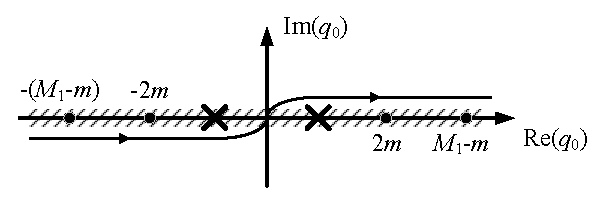
\includegraphics[scale=1.5]{PathIntegrateMode2.eps}
		\caption{Контур интегрирования по $q_0$ в~(\ref{eq:FullIntegrate}) для моды 2. Штрихами показана область нестабильности фотона. Крестиком обозначен полюс, соответствующий $q_0=\omega$ -- вещественному собственному значению поляризационного оператора.}\label{fig:FullPathIntegr}.
	\end{figure}

Контур интегрирования $C$ определяется согласно аналитическим свойствам подынтегрального выражения. В частности, в точке $q_0=\omega$ подынтегральное выражение~(\ref{eq:FullIntegrate}) имеет полюс, который соответствует уравнению дисперсии:

\begin{equation}
	\omega^2 - \vec{k}^2 - {\cal P^{(\lambda)}}(q)=0.
\end{equation}

С другой стороны, как было показано в работе~\cite{MikhChist:2001}, собственные значения поляризационного оператора как в магнитном поле, так и в замагниченной плазме помимо полюсов $q_{\mprl}^2=(M_n\pm M_\ell)^2$, отмеченных в главе 1 настоящей диссертации, также имеют разрезы, которые связаны с распадом фотона на $e^+e^-$-пару и переходом электрона на другие уровни Ландау, т. е. соответствуют областям нестабильности фотона (см. рис.~\ref{fig:FullPathIntegrMode1} и~\ref{fig:FullPathIntegr}). С учетом этих особенностей  контур интегрирования может быть определен, как показано на~рис.~\ref{fig:FullPathIntegrMode1}~и~\ref{fig:FullPathIntegr}.

Следует отметить, что в сильно замагниченной плазме в кинематической области $q_0<2m$ мнимая часть поляризационного оператора для обеих мод пренебрежимо мала по сравнению с реальной частью (влияние резонансов отсутствует), поэтому для удобства контур интегрирования как для фотона моды~1, так и для фотона моды 2 можно преобразовать согласно рис.~\ref{fig:PathIntegr}. Таким образом, интеграл~(\ref{eq:FullIntegrate}) можно представить в виде двух слагаемых
\begin{eqnarray}
F^{(\lambda)}(t) = F^{(\lambda)}_{pole}(t) + F^{(\lambda)}_{cut}(t),
\label{eq:19}
\end{eqnarray}
%
первое из которых определяется вычетом в точке $q_0 = \omega$, являющейся
решением уравнения дисперсии $q^2 - {\cal P}^{(\lambda)}(q) = 0$ в кинематической области, где собственное 
значение поляризационного оператора фотона ${\cal P}^{(\lambda)}(q)$ -- вещественно. 

%Оно соответствует незатухающему
%решению в области $\omega < 2 m$~\cite{Shab}.
Второе слагаемое определяет зависимость потенциалов ${\cal A}^{(\lambda)}_\alpha(x)$ от времени
в области $q_0>2m$ и имеет вид
фурье-интеграла:
%
\begin{eqnarray}
F^{(\lambda)}_{cut}(t) &=& \int \limits_{- \infty}^{\infty} \frac{dq_0}{2 \pi}\,
F^{(\lambda)}_{cut}(q_0)e^{- i q_0 t},
\label{eq:20} 
\\
F^{(\lambda)}_{cut}(q_0) &\simeq& 
\frac{2 \,\theta (q_0  -  2 m)\,I^{(\lambda)}}
{q_0\,([ q_0^2 - {\bf k}^2 - R^{(\lambda)}]^2 + [I^{(\lambda)}]^2)},
\label{eq:21}
\end{eqnarray}
%
где $R \equiv \text{Re} {\cal P}^{(\lambda)}(q_0)$  – реальная, $I \equiv  - \text{Im} {\cal P}^{(\lambda)}(q_0 + i \varepsilon)$ – мнимая 
части поляризационного оператора фотона в замагниченной плазме.
\newpage
Мнимая часть поляризационного оператора может быть получена из коэффициента  
поглощения фотона и представлена в следующем виде:
\begin{eqnarray}
W^{(\lambda)}_{abs} = W_{\gamma^{(\lambda)} \to e^+ e^-} + W_{\gamma^{(\lambda)} e^{\pm} \to e^{\pm}} \, .
\label{eq:Wabs}
\end{eqnarray}
где $W_{\gamma^{(\lambda)} \to e^+ e^-}$ -- коэффициент поглощения фотона в процессе однофотонного рождения электрон-позитронной пары, $W_{\gamma^{(\lambda)} e^{\pm} \to e^{\pm}}$ -- коэффициент поглощения фотона в процессе поглощения фотона электроном.

\begin{figure}[t]\centering
	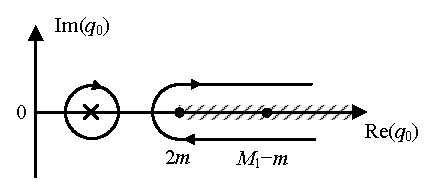
\includegraphics[scale=1.5]{PathIntegrate2Gl.eps}
	\caption{Контур интегрирования по $q_0$ в~(\ref{eq:20}) для мод $\lambda = 1,2$. Штриховой линией показана область, где мнимая часть поляризационного оператора двух возможных мод $\lambda = 1,2$ существенна. Остальные обозначения аналогичны~рис.~\ref{fig:FullPathIntegr}.}\label{fig:PathIntegr}
\end{figure}

С учетом процессов излучения фотонов, (\ref{eq:Wabs}) может быть представлена в следующей форме (см., например,~\cite{Shabad:1988, Rumyantsev:2017,Weldon:1983}): 
\begin{eqnarray}\label{eq:Ilambda}
I^{(\lambda)}=\text{Im} {\cal P}^{(\lambda)} =  -2 q_0 [1-\exp (-q_0/T)] W^{(\lambda)}_{abs} \, . 
\label{eq:ImP}
\end{eqnarray}

Значения $W_{\gamma^{(1)} \to e^+ e^-}$ могут быть получены из~(\ref{eq:wabs1})
с использованием перекрестной симметрии:
\begin{equation}\label{eq:Wgamma1epem}
	\begin{gathered}
		W_{\gamma^{(1)}\to e^+e^-}= \frac{\alpha\beta }{q_0}\sum_{\ell, \ell'=0}^{\infty}\frac{[1-f_{E_{\ell}}][1-f_{q_0-E_\ell}]}{\sqrt{\left( M_{\ell'}^2-M_\ell^2-q_0^2\right)^2-4q_0^2 M_\ell^2}}\times
		\\
		\times \left\{\left(2\beta  ({\ell'}+\ell)-q_0^2\right)\left({\cal I}_{{\ell'},\ell-1}^2+{\cal I}_{{\ell'}-1,\ell}^2\right)-
		8 \beta  \sqrt{l n} {\cal I}_{{\ell'},\ell} {\cal I}_{{\ell'}-1,\ell-1}
		\right\}\, ,
	\end{gathered}
\end{equation}
где ${\cal I}_{n, \ell}\equiv{\cal I}_{n, \ell}(\frac{q_\perp^2}{2\beta})$.

\newpage
Из~(\ref{eq:Wgamma1epem}) следует, что для фотона моды 1 коэффициент поглощения для процесса рождения электрон-позитронной пары на уровнях Ландау $\ell=\ell'=0$ равен нулю. Для фотона моды 2 из~(\ref{eq:wabs2}) получим:
\begin{equation}
\begin{gathered}
%W_{\gamma^{(2)}\to e^+e^-}=\frac{\alpha\beta}{2}\frac{1}{M_{\ell'}q_0^2}\frac{1}{q_0\sqrt{(q_0^2-(M_\ell^2+M_{\ell'}^2))^2-4M_\ell^2M_{\ell'}^2}}\frac{1}{q_0^2-(M_\ell+M_{\ell'})^2}\times
%\\
%\times\bigg(
%(q_0^2+(M_\ell^2-M_{\ell'}^2))^2 M_{\ell'}(M_\ell^2+M_{\ell'}^2+2m^2)
%-
%2M_\ell (M_\ell+M_{\ell'})^2(m^2+3M_\ell M_{\ell'})q_0^2\bigg)\times
%\\
%\times[{\cal I}_{\ell,\ell'}^2+{\cal I}_{\ell-1,\ell'-1}^2] - 4M_{\ell'} q_0^2 (q_0^2-(M_\ell+M_{\ell'})^2)2\beta \sqrt{\ell \ell'} {\cal I}_{\ell\ell'} I_{\ell-1,\ell'-1}\\
W_{\gamma^{(2)}\to e^+e^-}= \frac{\alpha\beta }{q_0}\sum_{\ell, \ell'=0}^{\infty}\frac{[1-f_{E_\ell}][1-f_{q_0-E_\ell}]}{\sqrt{\left( M_{\ell'}^2-M_\ell^2-q_0^2\right)^2-4q_0^2 M_\ell^2}}\times
\\
\times \left\{\left(\frac{\left[2\beta  ({\ell'}-{\ell'})\right]^2}{q_0^2}-2 \beta  (\ell+{\ell'})-4m^2\right)\left({\cal I}_{{\ell'},\ell}^2+{\cal I}_{{\ell'}-1,\ell-1}^2\right)-
8 \beta  \sqrt{\ell {\ell'}} {\cal I}_{{\ell'},\ell} {\cal I}_{{\ell'}-1,\ell-1}
\right\}\, .
\end{gathered}
\end{equation}


Реальная часть 
поляризационного оператора может быть восстановлена по его мнимой части с помощью дисперсионного соотношения с одним 
вычитанием:
%
\beq 
R^{(\lambda)}=\textrm{Re}{\cal P}^{(\lambda)} (t) = \int \limits_0^\infty \frac{\textrm{Im}({\cal P}^{(\lambda)} (t'))\,dt'}{t'-t-i o} - \textrm{Re}{\cal P}^{(\lambda)} (0)\,, \qquad  t = q^2_0 \, .
\label{eq:Disp}
\eeq

В общем случае произвольных уровней Ландау $\ell$ и $\ell'$ задача о вычислении $\textrm{Re} {\cal P}^{(\lambda)}(t)$ выглядит очень громоздко, поэтому в сильно замагниченной плазме можно ограничиться вкладом только первых двух уровней Ландау, которые для области $q_0>2m$ будут выглядеть следующим образом:
\beq
&&W_{\gamma^{(1)} e \to e} \simeq \frac{\alpha \beta}{q_0}
%\times 
%\\
%\nonumber
%&&\times 
\frac{f_{E_{0}} (1 - f_{E_{0} + q_0})}{\sqrt{(2\beta-q^{2}_{0})^2-4 q^{2}_{0}m^2}} (2 \beta - q^{2}_{0}) e^{-\frac{q_0^2}{2\beta}}   \, ,
\eeq
%

\beq
\label{eq:wabs2} 
&&W_{\gamma^{(2)} e \to e} \simeq
\frac{\alpha \beta}{q_0} 
%\times 
%\\
%\nonumber
%&&\times 
\frac{f_{E_{0}} (1 - f_{E_{1} + q_0})}{\sqrt{(2\beta-q^{2}_{0})^2-4 q^{2}_{0}m^2}}
\left (\frac{4\beta^2}{q^{2}_{0}} - 2 \beta - 4 m^2 \right )
\frac{q_0^2}{2\beta} e^{\frac{q_0^2}{2\beta}}\, ,
\eeq
\begin{equation}\label{eq:Wgam2ee}
	\begin{aligned}
			&W_{\gamma^{(2)} \to e^+e^-} \simeq\frac{\alpha \beta}{q_0}e^{\frac{q_0^2}{2\beta}} \bigg\{
		\frac{(1-f_{E_{0}}) (1 - f_{q_0 - E_{0}})}{q_0\sqrt{q^{2}_{0}-4 m^2}}
		\left (- 4 m^2 \right )+
		\\
		& 
		+
		\frac{q_0^2}{\beta}
		%\times 
		%\\
		%\nonumber
		%&&\times 
		\frac{(1-f_{E_{0}}) (1 - f_{q_0 - E_{1}})}{\sqrt{(2\beta-q^{2}_{0})^2-4 q^{2}_{0}m^2}} 
		\left (\frac{4\beta^2}{q^{2}_{0}} - 2 \beta - 4 m^2 \right ) 
		%\times 
		%\\
		%\nonumber
		%&& \times 
		 \bigg\} \, ,
	\end{aligned}
\end{equation}
где
\beq
\nonumber
&&E_{n} = \frac{1}{2 q_{0}} \,\left|2\beta n - q^2_{0}\right |\, .
\eeq

В результате выражения для мнимой и действительной частей поляризационного оператора для фотонов моды 1 и моды 2 с учетом~(\ref{eq:Ilambda}--\ref{eq:Wgam2ee}) и магнитного поля при условии $q_0^2>4m^2$ удобно представить следующим образом:

\begin{equation}
I^{(1)}=2\alpha\beta\exp \left[-\frac{q_\perp^2}{2\beta }\right]\frac{\left(2\beta -q_0^2\right) f_{E_0}\left(1-f_{E_0+q_0}\right)\left(1-\exp[q_0/T]\right)}{ \sqrt{\left((M_1-m)^2-q_0^2\right) \left((M_1+m)^2-q_0^2\right)}}
\end{equation}

\begin{equation}\begin{aligned}
R^{(1)}&= -\frac{\alpha \beta}{2\pi}\exp\left[\frac{-q_\perp^2}{2\beta}\right]\bigg(\frac{M_1^2-m^2-q_0^2}{\sqrt{((M_1+m)^2-q_0^2)((M_1-m)^2-q_0^2)}}
\times
\\
&\times
\ln\left[\frac{\sqrt{(M_1+m)^2-q_0^2}+\sqrt{(M_1-m)^2-q_0^2}}{2\sqrt{M_1 m}}\right]-\ln\left[\frac{M_1^2}{m^2}\right]\bigg)
-
\\
&-\frac{\alpha \beta q_0^2 m^2}{2\pi} \exp\left[-\frac{q_\perp^2}{2\beta}\right]\int_{0}^{\infty}\frac{\dd z}{\exp \left[\frac{m}{T}\sqrt{z^2+1}\,\right]+1}\times
\\
&\times\frac{\sqrt{z^2+1}}{ \left(M_1^2-m^2-q_0^2\right)^2-4m^2q_0^2 \left(z^2+1\right)}\, ,
\end{aligned}
\end{equation}

\begin{equation}\begin{aligned}
I^{(2)}=&-2\alpha\beta\left(1-\exp\left[{\frac{-q_0}{T}}\right]\right)\exp\left[{\frac{-q^2_\perp}{2\beta}}\right] \bigg\{
\frac{(1-f_{E_{0}}) (1 - f_{q_0 - E_{0}})}{q_0\sqrt{q^{2}_{0}-4 m^2}}
\left (- 4 m^2 \right )+
\\
& 
+
\frac{q_0^2}{\beta}
%\times 
%\\
%\nonumber
%&&\times 
\frac{4\beta^2/q^{2}_{0} - 2 \beta - 4 m^2}{\sqrt{((M_1+m)^2-q_0^2)((M_1-m)^2-q_0^2)}}\times
\\
&\times\bigg[(1-f_{E_{0}}) (1 - f_{q_0 - E_{1}})+
\frac{1}{2}f_{E_{0}} (1 - f_{E_{1} + q_0})
\bigg]
\bigg\}\, ,
\end{aligned}\end{equation}

\begin{equation}\begin{aligned}
	R^{(2)}&= \frac{\alpha\beta}{2\pi}\exp\left[-\frac{q_\perp^2}{2\beta}\right]\left(\frac{4m^2}{\sqrt{q_0^2(q_0^2-4m^2)}}\ln\left[\frac{\sqrt{q_0^2}+\sqrt{q_0^2-4m^2}}{4m^2}\right]+1\right)+ 
	\\
	&+\frac{\alpha}{16\pi}q^2_\perp \exp\left[-\frac{q_\perp^2}{2\beta}\right] \bigg( \frac{4m^2+2\beta+\frac{4\beta^2}{ q_0^2}}{\sqrt{((M_1-m)^2-q^2_0)((M_1-m)^2-q^2_0)}}
	\times
	\\
	&\times
	\ln\left[\frac{\sqrt{(M_1+m)^2-q_0^2}+\sqrt{(M_1-m)^2-q_0^2}}{2(m^4+2\beta m^2)^{1/4}}\right]+
	\\
	&+\frac{1}{2}\left(\frac{m^2}{\beta}-\frac{2\beta}{q_0^2}\right)\ln\left[\frac{m^2+2\beta}{m^2}\right]+1\bigg)- \frac{4\alpha\beta m^2}{\pi}\exp\left[-\frac{q_\perp^2}{2\beta}\right]\times
	\\
	&\times
	\int_{0}^{\infty}\frac{1}{\sqrt{1+z^2}}\frac{1}{\exp[\frac{m}{T}\sqrt{(1+z^2)}\,]+1}\bigg(\frac{1}{q_0^2-4m^2(1+z^2)}+
	\\
	&+\frac{q_0^2}{\beta}\frac{2\beta z^2 + q_0^2}{(2\beta - q_0^2)^2-m^2(1+z^2)q_0^2}\bigg)\dd z\, .
\end{aligned}\end{equation}

Следует отметить, что в поставленной задаче рассматриваются процессы только до второго циклотронного резонанса $q_0=M_1-m$, поэтому те же процессы с другими уровнями Ландау вклада не дают.

Выражения (\ref{eq:20})-(\ref{eq:Wabs}) с учетом (\ref{eq:Disp}) решают задачу 
о нахождении временной зависимости волновой функции фотона  в присутствии сильно 
замагниченной плазмы. 

\begin{figure}[t!]\centering
	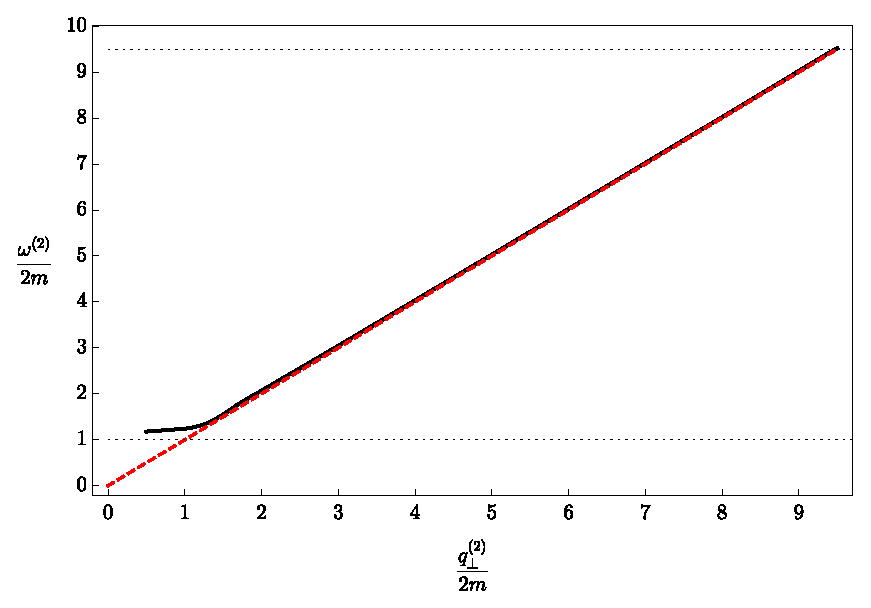
\includegraphics[scale=1.2]{DisperseMode2.eps}
	\caption{Дисперсия фотона моды 2 в области нестабильности, связанной с процессами распада на $e^+e^-$ пару и поглощения $e_0 \gamma^{(2)}\to e_1$, представлена сплошной линией при магнитном поле $B=200B_e$ и $T=1$~МэВ. Штриховая линия соответствует вакуумному закону дисперсии. Пунктирные линии обозначают пороги $\omega^{(2)}=2m$ и $\omega^{(2)}=M_1-m$. \label{fig:DisperseMode2}}
\end{figure}

Временную часть волновой функции фотона $F(t)$ можно представить в виде затухающих колебаний для мод $\lambda=1,2$:
\begin{equation}\label{eq:Fm}
	F^{(\lambda)}(t)\sim F^{(\lambda)}_A(t) \cos(\omega^{(\lambda)} t+\phi_0)
\end{equation}
где $F^{(\lambda)}_A(t)$ -- амплитуда колебаний,
временная зависимость которой определяет
характер затухания волновой функции,
$\omega^{(\lambda)}$ -- эффективная
частота. В работе~\cite{Shabad:1988}
предполагался экспоненциальный характер затухания с декрементом затухания, равным мнимой части энергии фотона, полученным из решения уравнения дисперсии на втором римановом листе. Анализ  аналитических свойств фурье-образа $F^{(\lambda)}_{cut}(q_0)$ показывает, что характер временного затухания волновой функции в общем случае является неэкспоненциальным. Тем не менее на протяжении некоторого характерного отрезка времени $(\sim [W^{(\lambda)}_{abs}]^{-1})$
зависимость волновой функции от времени можно приближенно описать как 
экспоненциально затухающие гармонические колебания:
%
\begin{equation}\label{eq:ApproxA}
{\cal A}^{(\lambda)}_\mu(t) \sim e^{- \gamma^{(\lambda)}_\text{eff} \, t/2} \cos 
(\omega^{(\lambda)} t + \phi_0).
\end{equation}
%
Здесь $\omega^{(\lambda)}$ и $\gamma^{(\lambda)}_\text{eff}$ -- эффективная 
частота и коэффициент  
поглощения фотона моды $\lambda$ соответственно, которые должны быть найдены с использованием 
(\ref{eq:20})--(\ref{eq:Wabs}) для каждого значения импульса ${\bf k}$, что определяет эффективный 
закон дисперсии фотона в области его нестабильности~(см. рис.~\ref{fig:DisperseMode1} и \ref{fig:DisperseMode2}).


\section{Численный анализ}



\begin{figure}[t]\centering
	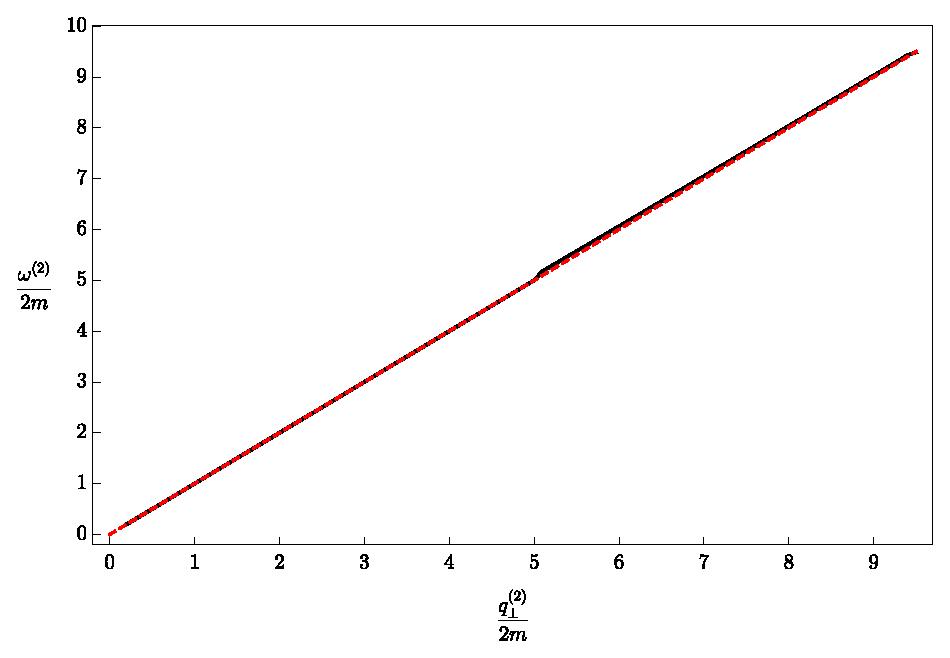
\includegraphics[scale=1.2]{DisperseMode1.eps}
	\caption{Дисперсия фотона моды 1 в области нестабильности, связанной с процессом поглощения $e_0 \gamma^{(1)}\to e_1$ представлена при магнитном поле $B=200B_e$ и $T=1$~МэВ. Пунктирная линия обозначает порог $\omega^{(1)}=M_1-m$ \label{fig:DisperseMode1}}
\end{figure}

Рис.~\ref{fig:DisperseMode1} и ~\ref{fig:DisperseMode2} демонстрируют законы дисперсии фотонов моды 1 и моды~2 в сильно замагниченной плазме при температуре $T = 1$ МэВ и магнитном поле $B = 200B_e$ в области их нестабильности. Из представленных результатов следует, что закон дисперсии для фотона моды 1 в области нестабильности незначительно отличается от вакуумного закона дисперсии~(см.~рис.~\ref{fig:DisperseMode1}). С другой стороны, дисперсионная кривая фотона моды 2 значительно отличается от вакуумной вблизи порога $\omega^{(2)}=4m$ и в малой окрестности порога~$\omega^{(2)}=M_1-m$. Для построения дисперсионной кривой до следующего резонанса необходимо учитывать следующие уровни Ландау. При этом полученная картина дисперсионных кривых согласуется с анализом уравнения дисперсии, выполненного в работе~\cite{Shabad:1988}.


\begin{figure}[t]\centering
	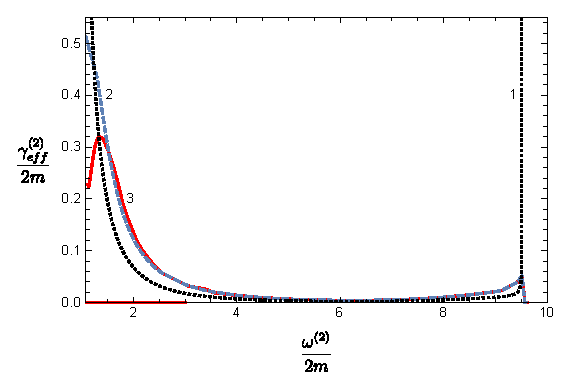
\includegraphics[scale=0.8]{mode2.eps}
	\caption{\label{fig:fig2}Зависимость ширины распада фотона моды 2 от частоты в припороговых областях при $B=200 B_e$, $T=1$ МэВ и $ \mu=0 $. Линия $ {\it 1} $ - коэффициент поглощения фотона $ W ^ {(1)}_{abs} $,
		% в процессах $ \ gamma \ to e ^ + e ^ - $ и $ \ gamma e ^ { \ pm} \ to e ^ {\ pm} $,
		вычисленный в древесном приближении и содержащий корневые особенности; линия $ {\it 2} $ - ширина распада, полученная из комплексного решения дисперсионного уравнения на втором римановом листе [6]; линия $ {\it 3} $ соответствует ширине затухания $ \gamma^{(1)}$, вычисленной на основе приближения~(\ref{eq:ApproxA}).}\label{fig:DampMode2}
\end{figure}

Для астрофизических приложений полезно вычислить величину $\gamma_\text{eff}$, которая определяет интенсивность поглощения 
$\gamma$-квантов в замагниченной плазме за счет  процессов $\gamma \to e^+ e^-$  и $\gamma e^{\pm} \to e^{\pm}$.
Обычно в астрофизике  используют выражение для коэффициента поглощения,
полученное на основе  вероятности распада  $ \gamma \to e^+ e^-$. Однако в околопороговой области эти выражения
содержат корневые сингулярности (см. например~\cite{HBG:1997}), которые были отмечены во введении к данной главе. 

\newpage
Наш анализ показывает, (см. рис.~\ref{fig:DampMode1} и~\ref{fig:DampMode2}),
что вычисление коэффициента  поглощения с учетом неэкспоненциального характера 
затухания приводит к конечному выражению для коэффициента  поглощения фотона в окрестности резонансов 
$q_0 = (\sqrt{m^2+2 \beta} - m )$ как для фотона моды 2, так и для фотона моды 1. Исходя из рис. \ref{fig:DampMode1} можно сделать вывод, что фотон моды 1 является квазистабильным в областях $q_0<7$ МэВ и $q_0>(\sqrt{m^2+2 \beta} - m)\simeq 9.5$~МэВ. С другой стороны, фотон неустойчив в области, близкой в окрестности резонансов $q_0 = (\sqrt{m^2+2 \beta} - m )$. Фотон моды 2 можно считать квазиустойчивым в области $q_0<4m$ и $q_0>(\sqrt{m^2+2 \beta} - m)$. Коэффициент затухания фотона, полученный из результатов работы~\cite{Shabad:1988}, является завышенным в околопороговой области по сравнению с результатами, полученными с помощью аппроксимации~(\ref{eq:ApproxA}). Однако существует область энергий фотона ($2.5\lesssim q_0\lesssim 8.5$ МэВ для фотона моды 2 и $q_0\lesssim8.7$ МэВ для фотона моды 1), где коэффициенты поглощения, полученные из результатов работы~\cite{Shabad:1988} и с помощью аппроксимации~(\ref{eq:ApproxA}) совпадают.


\begin{figure}[t]\centering
	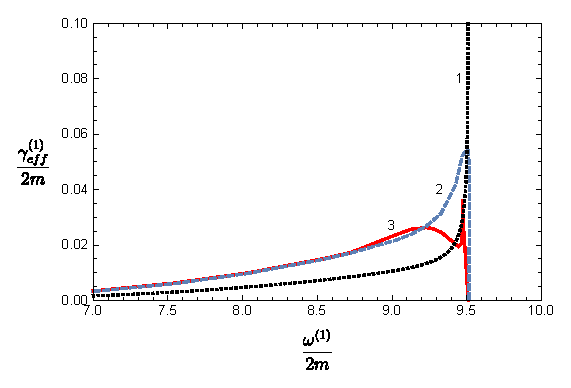
\includegraphics[scale=0.8]{mode1.eps}
	\caption{\label{fig:fig1}Зависимость ширины распада фотона моды 1 от частоты в припороговых областях при $B=200 B_e$, $T=1$ МэВ и $ \mu=0 $. Линия $ {\it 1} $ - коэффициент поглощения фотона $ W ^ {(1)}_{abs} $,
		% в процессах $ \ gamma \ to e ^ + e ^ - $ и $ \ gamma e ^ { \ pm} \ to e ^ {\ pm} $,
		вычисленный в древесном приближении и содержащий корневые особенности; линия $ {\it 2} $ - ширина распада, полученная из комплексного решения дисперсионного уравнения на втором римановом листе [6]; линия $ {\it 3} $ соответствует ширине затухания $ \gamma^{(1)}$, вычисленной на основе приближения~(\ref{eq:ApproxA}).}\label{fig:DampMode1}
\end{figure}

\begin{figure}[t!]\centering
	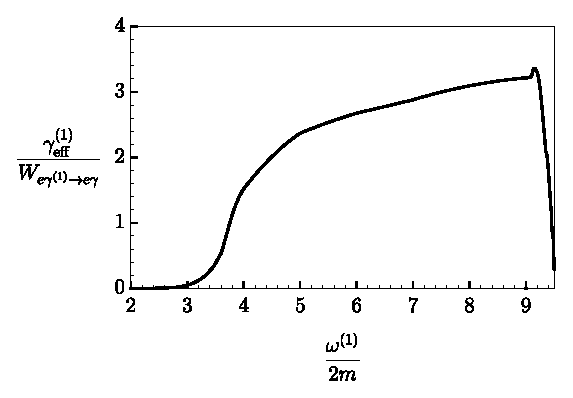
\includegraphics[scale=1.3]{CompareDampAndCompton.eps}
	\caption{\label{fig:ComptonandDamp} Отношение коэффициента затухания фотона $\gamma_{eff}^{(1)}$ к коэффициенту поглощения фотона в процессе $e\gamma^{(1)}\to e\gamma$ при $B=200B_e$ и $T=1$ МэВ}
\end{figure}
\begin{figure}[t!]\centering
	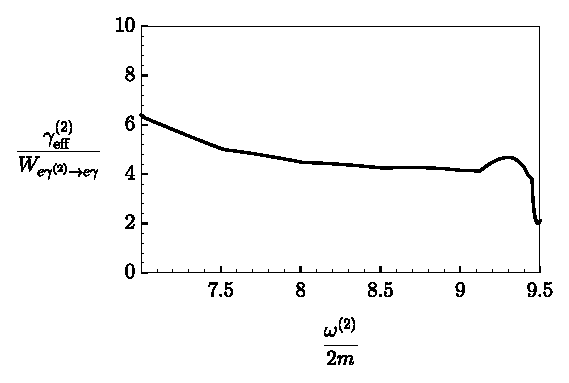
\includegraphics[scale=1.3]{CompareDampAndCompton2.eps}
	\caption{\label{fig:ComptonandDamp2} Отношение коэффициента затухания фотона $\gamma_\text{eff}^{(2)}$ к коэффициенту поглощения фотона в процессе $e\gamma^{(2)}\to e\gamma$ при $B=200B_e$ и $T=1$ МэВ}
\end{figure}
\clearpage

На основе полученных результатов представляет интерес рассмотреть задачу о возможности формировании комптоновского процесса при условии затухания фотона. Для этого удобно вычислить отношение коэффициента затухания фотона к коэффициенту поглощения фотона $e\gamma^{(1)}\to e\gamma$  (см. рис. \ref{fig:ComptonandDamp}), полученном в главе 2 и который определяет время его формирования. Как видно из рисунка~\ref{fig:ComptonandDamp}, комптоновский процесс, несмотря на малый фактор $\alpha$, успевает формироваться при энергиях фотона $\omega\lesssim3$ МэВ. Для фотона моды 2 комптоновский процесс формируется только в области энергий фотона $\omega\lesssim1$ МэВ. В области энергий $\omega>3$ МэВ для моды 1 и $\omega>1$ МэВ фотоны будут эффективно затухать, и комптоновский процесс, по-видимому, не успевает сформироваться. Для моды 2 (см. рис.~\ref{fig:ComptonandDamp2}) даже с учетом области квазистабильности (вдали от порогов), комптоновский процесс будет формироваться только при энергиях фотона~$\omega<1$~МэВ.

Таким образом, коэффициенты поглощения фотона в комптоновском процессе для двух возможных каналов рассеяния $e\gamma^{(1)}  \to e\gamma^{(1)}$ и $e\gamma^{(1)}  \to e\gamma^{(2)}$, несмотря на резонансный характер, целесообразно рассматривать лишь вдали от циклотронных резонансах, поэтому для анализа комптоновского процесса при высоких температурах $T\simeq 1$ МэВ и магнитных полях $B=200 B_e$ достаточно использовать разложение по обратным степеням напряженности магнитного поля~\cite{Chistyakov:2009}. Каналы же рассеяния $e\gamma^{(2)}  \to e\gamma^{(1)}$  и $e\gamma^{(2)}  \to e\gamma^{(2)}$ в области резонанса рассматривать нецелесообразно, так как комптоновский процесс не успевает сформироваться для энергий фотона $\omega\gtrsim 2m$.

\newpage

\section{Выводы}
Исследован процесс распространения квантованной электромагнитной волны в сильно замагниченной, зарядово-симметричной плазме. С учетом изменения дисперсионных свойств фотона в магнитном поле и плазме было установлено, что, аналогично случаю чистого магнитного поля процесс затухания фотона
в замагниченной плазме имеет неэкспоненциальный характер. 

Для характерного отрезка времени $\sim [W^{{(\lambda)}}_{abs}]^{-1}$ была использована аппроксимация экспоненциально затухающими колебаниями. В этом случае было
показано, что коэффициент поглощения фотона в околопороговой области меньше по сравнению с известными в литературе результатами. Также, следуя данной аппроксимации, были построены дисперсионные кривые, которые и для моды 1, и для моды 2 близки к вакуумным кривым, за исключением околопороговых областей. Полученные результаты согласуются с выводами работы~\cite{Shabad:1988}.

Для определения характера затухания фотона необходимо выполнить более детальный анализ временной зависимости амплитуды $F_A(t)$ колебаний, входящей в уравнение~(\ref{eq:Fm}). Кроме того, был выполнен анализ возможности формирования комптоновского процесса в условиях нестабильности фотона за счет процесса поглощения электроном $e^\pm\gamma\to e^\pm$ и распада на электрон-позитронную пару $\gamma\to e^+e^-$. Несмотря на малый фактор $\alpha$, комптоновский процесс преобладает над процессами распада и поглощения в области низких энергий фотона ($\omega<3$ МэВ при $T=1$ МэВ и $B =200B_e$). С другой стороны, даже с учетом резонанса на виртуальном электроне, фотоны как моды 1, так и моды~2 в пределе сильного магнитного поля $B=200 B_e$ и температуре $T=1$ МэВ эффективно затухают в резонансной области.

%%%%%%%%%%%%%%%%%%%%%%%%%%%%%%%%%%%%%%%%%%%%%%%%%%%%%%%%%%%%%%%%%%%%

\section{Сингулярности в фазовых объемах одновершинных процессов и методы их устранения.}
\input{Chapter7}	
%%%%%%%%%%%%%%%%%%%%%%%%%%%%%%%%%%%%%%%%%%%%%%%%%%%%%%%%%%%%%%%%%%%%
\section{Заключение}
\input{conclusion}
%%%%%%%%%%%%%%%%%%%%%%%%%%%%%%%%%%%%%%%%%%%%%%%%%%%%%%%%%%%%%%%%%%%%
\newpage
\inputencoding{cp1251}
%\bibliography{mybib}
\bibliographystyle{gost705}
\bibliography{Bib}
\inputencoding{utf8}
\end{document}



В пропагаторе виртуального фермиона имеется конструкция вида:
%
\begin{eqnarray}
\frac{1}{p^{2}_{\mprl} - m_f^2 - 2\beta n - \Re^{s}_\Sigma (p) + \ii\, \Im^{s}_\Sigma (p)}\, .
\end{eqnarray}
%
Возникающие в знаменателе пропагатора реальная $\Re^{s}_\Sigma (p)$ и мнимая $ \Im^{s}_\Sigma (p)$ части, соответствующие поляризационному состоянию $s$, есть результат вычисления радиационных поправок 
к массе фермиона в замагниченной плазме. Мнимая часть  $\Im^{s}_\Sigma (p)$ может быть получена с помощью оптической теоремы 
и представлена в следующем виде~\cite{MGU, Zhukovskii:1994}:
%
\begin{eqnarray}
\Im^{s}_\Sigma (p) = - \frac{1}{2}\, p_0 \; \Gamma_n^{s} \, ,
\label{eq:I_Sigma}
\end{eqnarray} 
\noindent где $\Gamma_n^{s}$ -- вероятность изменения состояния фермиона, находящегося 
в поляризационном состоянии $s$ и занимающего  $n$-й уровень  Ландау.

Реальная часть массового оператора ${\cal R}^{s}_\Sigma (p)$ определяет изменение (по сравнению с вакуумным) 
закона дисперсии фермиона в присутствии замагниченной плазмы. В слабых магнитных полях, $B\ll B_e$, она определяется 
отношением~\cite{Ritus1969}:

\begin{eqnarray}
\label{Re1}
\Re^{s}_\Sigma (p) = \frac{4\alpha m_f}{3\pi} \varkappa^2 \left [ \ln \varkappa^{-1} + C + \frac{1}{2} \ln 3 - \frac{33}{16} \right],\quad \varkappa\ll 1,
\end{eqnarray}
\noindent где $C = 0.577...$ - постоянная Эйлера, динамический параметр $\varkappa$ вводится следующим образом:
%
\begin{eqnarray}
\varkappa = \frac{1}{m_f B_e} [-(F_{\mu\nu} p_{\nu})^2]^{1/2}.
\end{eqnarray}

В сильных магнитных полях, $B\gtrsim B_e$, сдвиг массы фермиона в основном состоянии описывается дважды 
логарифмической асимптотикой~\cite{Jancovici}:
%
\begin{eqnarray}
\label{Re2}
\Re^{s}_\Sigma (p) = \frac{\alpha}{4\pi} m_f \ln^2 (2\beta).
\end{eqnarray}

Из (\ref{Re1}) и (\ref{Re2}) следует, что как в слабых, так и в относительно сильных ($B_e \lesssim B\lesssim 10^{16}$~Гс) магнитных полях
поправка к массе фермиона, обусловленная вкладом $\Re^{s}_\Sigma (p)$, оказывается несущественной~\cite{KM_Book_2003,Sokolov:1986}.

Резонанс на фиртуальном фермионе имеет место быть в условиях, при которых возбуждаются высшие  ($n > 0$) уровни Ландау виртуального фермиона. При этом возможна ситуация, при которой реальная часть знаменателя
пропагатора виртуального фермиона обращается в ноль. В этом случае виртуальный фермион становится реальным с определённым законом дисперсии, находится на массовой поверхности. Амплитуда процесса с участием
виртуального фермиона в промежуточном состоянии при этом значительно увеличивается и определяется мнимой частью массового оператора~(\ref{eq:I_Sigma}). 

Среди резонансных процессов особый интерес представляют одно-, двух- и трёхвершинные процессы, поскольку существенное влияние на характеристики астрофизических процессов
будут оказывать только реакции, дающие лидирующие по константам связи вклады.
	
{\bf Одновершинные процессы}, будучи в замагниченной среде, становятся кинематически разрешены. Особенностью данных процессов можно отметить жесткие кинематические ограничения. Одним из таких процессов является \textit{процесс рождения фотона} $e\to e\gamma $, также называемый циклотронным или синхотронным излучением.  При высоких магнитных полях излучение обусловлено переходами на более низкие уровни Ландау. Следует отметить, 
что при очень сильных магнитных полях, когда $\beta\sim0.2$, электроны, находящиеся на более высоких уровнях Ландау, переходят непосредственно на основной уровень, а не на соседний. С другой стороны обратный к процессу рождения фотона \textit{процесс поглощения фотона} $e\gamma \to e$  приводит к переходу электрона на высшие уровни Ландау. Другой немаловажный квантовый процесс является \textit{Процесс однофотонного рождения электрон-позит\-ронной пары} $\gamma \to e^+e^-$. Особенностью данного процесса является то, что фотон эффективно распадается вблизи точек циклотронного резонанса, где поляризационный оператор фотона имеет сингулярности. 
Однако является подавленным в области ниже порога рождения $\hbar \omega = 2mc^2$.
		
{\bf Двухвершинные процессы.} Типичным примером двухвершинного процесса является {\bfseries комптоновский процесс}  $e \gamma \to e\gamma$. Вблизи циклотронных резонансов сечение комптоновского рассеяния, без учета 
конечной ширины поголощения электрона, становится бесконечным. В таком случае промежуточный (виртуальный) электрон становится реальным, т.е. его закон дисперсии соответствует массовой поверхности, 
а комптоновский процесс становится одновершинным процессом. Процесс обратного комптоновского рассеяния может быть эффективным механизмом генерации жёсткого рентгеновского излучения сильно замагниченных 
нейтронных звёзд. Учёт резонансов в процессе комптоновского рассеяния необходим при построении моделей остывания магнитаров.

Большое магнитное поле может индуцировать новые взаимодействия частиц. Таким образом могут возникать такие фотон-нейтринные процессы, как \textit{конверсия фотона в пару нейтрино-антинейтрино} 
$\gamma \to \nu \bar{\nu}$ или \textit{излучение фотона нейтрино} $\nu \to \nu \gamma$. Такие процессы имеют петлевую диаграмму с двумя виртуальными электронами и вершинами как слабого, так и электромагнитного взаимодействия. 
При плотностях порядка $\rho = 10^9$ г/см$^3$ начинают возбуждаться высшие уровни Ландау виртуального электрона в \textit{фотонейтринном комптоноподобном процессе} $\gamma e \to e\nu \bar{\nu}$,
в результате чего он приобретает резонансный характер. Это может приводить к увеличению эффективности этой реакции, вследствие чего она, наряду с $\gamma \to \nu \bar{\nu}$, может играть важную роль
 в остывании нейтронных звезд.
 
 Среди петлевых двухвершинных процессов особое место занимает поляризационный оператор фотона во внешнме поле. Именно он определяет изменение поляризационных и дисперсионных свойств фотона во внешней 
 активной среде . При изучении резонансных эффектов в магнитном поле и плазме оказывается важным учёт радиационных поправок к массе фермиона, что сводится к рассчёту массового оператора фермиона как ещё 
 одной петлевой двухвершинной диаграммы.
 
 Кроме этого, интерес представляют процессы с участием гипотетических частиц, таких как аксион -- наиболее веротяный кандидат на роль холодной тёмной материи. Возможным механизмом генерации 
 аксионов является резонансный процесс фоторождения на заряженных компонентах среды, $i \to f + a$.
		
{\bf Трехвершинные процессы.} Кроме того в остывании нейтронных звёзд также играет роль трехвершинный	
\textit{процесс двухфотонной аннигиляции} $\gamma\gamma\to\nu \bar{\nu}$. Среди электромагнитных процессов не менее интересным процессом является 
\textit{процесс рождения электрон-позитронной пары} $\gamma e \to e e^+e^-$, который может быть достаточно эффективным для производства $e^+e^-$-плазмы, в то время, как стандартный механизм 
при аккуратном учете дисперсионных свойств фотонов становится невозможным. Данный процесс также интересен тем, что в нем наблюдаются резонансы как на виртуальном электроне, так и на виртуальном фотоне. 
С точки зрения формирования спектра нейтронных звёзд важным является учет трехвершинного \textit{процесса расщепления фотона} $\gamma \to \gamma \gamma$ и \textit{процесс слияния фотонов} 
$\gamma \gamma \to \gamma$, которые выступают, как механизм изменения числа фотонов. При определенных условиях эти процессы могут конкурировать с комптоновским процессом.  \\
